% Preamble
% ******************
\documentclass[a4paper,12pt]{report}
% margin
\usepackage[margin=2.5cm]{geometry}
% line spacing
\setlength{\parindent}{4em}
\setlength{\parskip}{1em}
\renewcommand{\baselinestretch}{1.5}
% citation
% \usepackage{cite}
% Subfolders
\usepackage{subfiles}
% Graphics
\usepackage{subcaption} % Note: Subcaption and subfig are alternatives
% \usepackage{subfig}
\usepackage{graphicx}
\usepackage{placeins} % For float barriers
\usepackage{adjustbox}
\graphicspath{{res/}{../res/}} % path variable for graphics folders
% other
\usepackage[utf8]{inputenc}
\usepackage{amsmath}
\usepackage{amsfonts}
\usepackage{amssymb}
\usepackage{hyperref}
\usepackage{cleveref}
\usepackage[bottom]{footmisc}
\usepackage{listings}
\usepackage{xcolor}

% ********
% For code style
\definecolor{codegreen}{rgb}{0,0.6,0}
\definecolor{codegray}{rgb}{0.5,0.5,0.5}
\definecolor{codepurple}{rgb}{0.58,0,0.82}
\definecolor{backcolour}{rgb}{0.95,0.95,0.92}

\lstdefinestyle{mystyle}{
    backgroundcolor=\color{backcolour},   
    commentstyle=\color{codegreen},
    keywordstyle=\color{magenta},
    numberstyle=\tiny\color{codegray},
    stringstyle=\color{codepurple},
    basicstyle=\ttfamily\footnotesize,
    breakatwhitespace=false,         
    breaklines=true,                 
    captionpos=b,                    
    keepspaces=true,                 
    numbers=left,                    
    numbersep=5pt,                  
    showspaces=false,                
    showstringspaces=false,
    showtabs=false,                  
    tabsize=2
}

\lstset{style=mystyle}

% ******************
\begin{document}{}
\begin{titlepage}
    \begin{center}
        \vspace*{0.5cm}

        \LARGE
        \textbf{An Exploration of Applied Semantic Image Segmentation}

        % \vspace{0.3cm}
        % Utilising 

        \vspace{1.0cm}
        \Large

        \textbf{Moritz Bergemann\\ 19759948}

        \vfill

        A thesis presented for the degree of\\
        Bachelor of Advanced Science (Computing) (Honours)

        \vspace{2.5cm}

        % \includegraphics[width=0.4\textwidth]{university}

        \large
        School of Electrical Engineering, Computing and Mathematical Sciences\\
        Curtin University\\
        Australia\\
        November 2022

    \end{center}
\end{titlepage}
% \maketitle
% \newpage

\thispagestyle{plain}
\begin{center}
    \Large
    \textbf{An Exploration of Applied Semantic Image Segmentation}

    \vspace{0.4cm}
    \large
    % Thesis Subtitle

    \vspace{0.4cm}
    \textbf{Moritz Bergemann\\ 19759948}

    \vspace{0.9cm}
    \textbf{Abstract}
\end{center}

Abstract goes here.

\newpage
\chapter*{Acknowledgements}
This thesis has been completed under the supervision of Dr Sonny Pham and Associate Professor Aneesh Krishna, both of whom have played an integral role in the success of the endeavour.

\noindent I also give my acknowledgements to Tanmay Singha, Kristian Rados, Max Barker, and Harry Walters, who have all aided greatly through constant discussion and exchange of ideas.

\newpage
\tableofcontents
\newpage
\listoffigures
\newpage
\listoftables
\newpage
\thispagestyle{empty}

% List of Acronyms
% UDA - Unsupervised domain adaptation
% 
% 

% ------------------------------------------------------------------------------
% Introduction?
% ------------------------------------------------------------------------------
\chapter{Introduction}
Semantic segmentation is a core task in computer vision that involves performing classification on every pixel in an input image. Unlike other computer vision tasks such as image classification (identifying which of a set of classes an input image belongs to) or object detection (identifying, classifying, and locating objects in an image), semantic segmentation provides highly dense and semantically rich information, particularly about the shapes objects take up and the intersections between objects.

\begin{figure}[h]
    \centering
    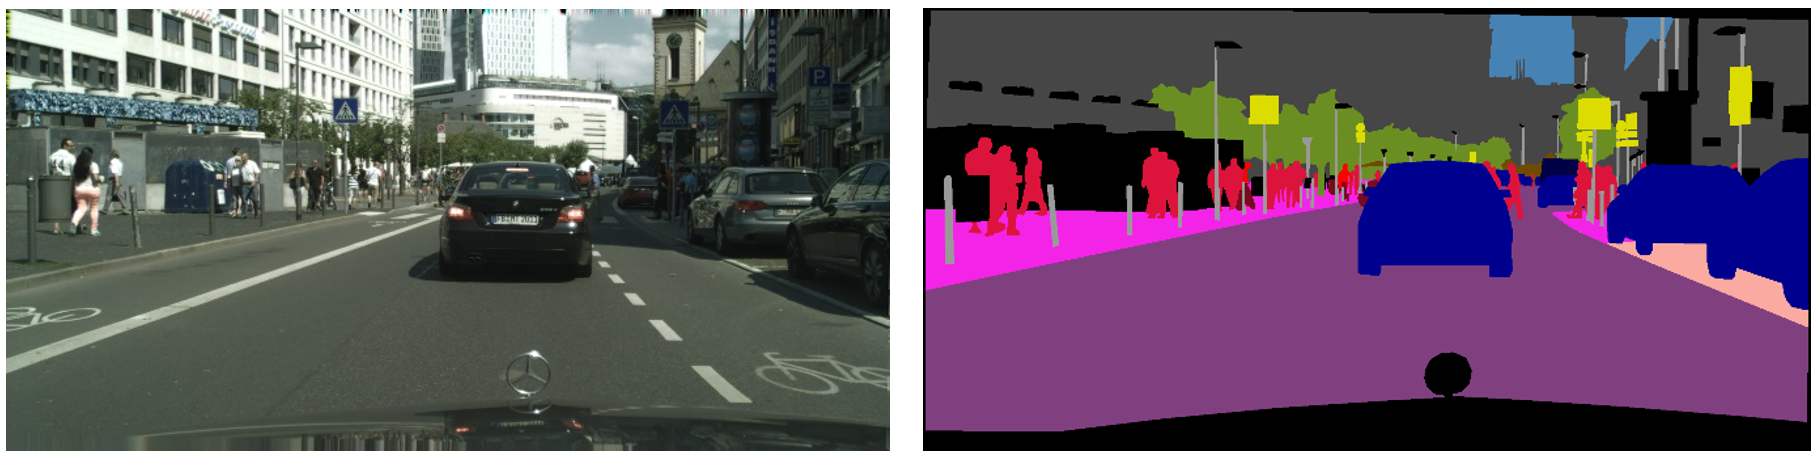
\includegraphics[width=\textwidth]{res/cityscapes-segmentation-sample.png}
    \caption{An example of an annotated semantic segmentation image from the Cityscapes dataset \cite{cordts_cityscapes_2016}. The left is the input to the model, and the right is the expected output.}
    \label{fig:cityscapes_segmentation_example}
\end{figure}

Segmentation is a key pre-processing task for many applications. Use in self-driving cars and robotics is most often cited. To safely drive, a self-driving car must be able to identify the shape, course, and edges of the road in front of it rather than only identifying it as a road, for instance. Medical analysis is another key segmentation task that can helps automate the essential task of medical identification and analysis. Many publications focus exclusively on the segmentation of CT or MRI images for medical applications \cite{hesamian_deep_2019}. Other applications include satellite mapping, video surveillance, augmented reality, damage detection, and domain transformation \cite{richter_enhancing_2021}.

Semantic segmentation is distinguished from other computer vision tasks through its density and computational complexity. Density is key in segmentation as the output is pixel-wise - therefore, a significant amount of information must be known about each pixel in the image to accurately segment it, especially for the boundaries between images. The increase in computational cost is also intuitive. No matter the scenario, generating an output that has the same dimensions as the model input will be more computationally intensive than a classification model that simply outputs a single vector. This, combined with the high complexity of producing training data for the segmentation task, means there has been significant research into effectively applying semantic segmentation to a number of relevant real-world domains, often with domain-specific applications being necessary. My research has been into one of these domains - structural crack segmentation - as well as the more general concept of semantic segmentation domain adaptation, which improves the ability to use existing labelled data to apply semantic segmentation to any domain.


\section{Motivation}
Semantic segmentation is a complex problem on many levels. Models that produce densely detailed output in general require specialised architectures, whether this is through an encoder-decoder approach that uses a traditional vision model as a backbone \cite{chen_deeplab_2017} or via a wholly unique architecture \cite{sandler_mobilenetv2_2019}. Additionally, the process of producing manually labelled pixel-level data for semantic segmentation (\autoref{fig:cityscapes_segmentation_example}) is extremely expensive and time-consuming compared to other tasks. The popular cityscapes dataset, for example, required over 1.5 hours of manual labelling for each of the 5000 finely labelled images \cite{cordts_cityscapes_2016}. Therefore, significant research has gone into the architecture and training level of semantic segmentation to improve its usability for real-world applications.

One aspect of research for applications is usage-specific architectures. Medical segmentation models, for example, may seek to maximise segmentation accuracy and detail without major focus on prediction time \cite{ronneberger_u-net_2015}, whereas areas where real-time segmentation is necessary, such as self-driving cars, may sacrifice some accuracy and detail in an architecture capable of producing many predictions per second \cite{poudel_fast-scnn_2019}. Structural crack segmentation is one such domain, where a relatively simple issue (segment only crack vs non-crack) requires fine resolution detail due to the thin nature of cracks, while also preferring efficient performance due to the large amount of data that must be processed. Therefore, one of the goals of this research was to investigate more performant efficient crack segmentation architectures.

Unsupervised domain adaptation (UDA) is a different means of applying segmentation to the real world. It involves taking the "knowledge" a segmentation model learns on one labelled dataset (e.g. Cityscapes) and applying it to an unlabelled task. While unlikely to be as effective as using labelled data, UDA can produce acceptable results in a new domain without the extremely expensive process of manually labelling data. In this research, we further investigate UDA for semantic segmentation, placing specific focus on segmentation transformer architectures as the transformer has been found to be extremely effective for domain adaptation tasks \cite{yang_tvt_2021} \cite{xu_cdtrans_2021} \cite{hoyer_daformer_2022}.


\section{Background}
This section will include a general review of semantic segmentation relevant to the research, with more specific background information appearing in the respective chapters.

As with most computer vision applications, deep convolutional neural networks (CNNs) have traditionally achieved state-of-the-art results on semantic segmentation tasks for accuracy and efficiency. The superior performance of CNNs is often cited to be due to their possession of vision-specific inductive biases. Translational equivariance means that patterns present anywhere in an image will be extracted in the same way due to the constant convolution kernel that “slides” across the input. Locality means that CNNs, due to the limited size of each kernel, will inherently put stronger weights towards input features that are closer together in 2D space (figure ~\ref{fig:receptive_field}) \cite{zhang_dive_2019}. All of this is achieved with fixed-size kernels, meaning the number of parameters that must be trained for any model does not increase with image size. Novel advances in general computer vision are typically first made on the simpler image classification task, then transferred to other tasks like segmentation.

Most semantic segmentation approaches follow some kind of encoder-decoder structure \cite{zhang_dive_2019}. This approach consists of two parts. First, the encoder maps the input sequence to an abstract representation, typically known as a feature space. Many segmentation models, starting with FCN (Fully Convolutional Network) \cite{long_fully_2015}, use an existing classification network, called the "backbone", for this feature extraction. The decoder is the second component, which reconstructs an output image from its feature representation, in this case into a segmentation map. U-Net \cite{ronneberger_u-net_2015}, ubiquitous in medical segmentation applications, is an early example of a backbone-less encoder-decoder for segmentation.

\begin{figure}[ht]
    \centering
    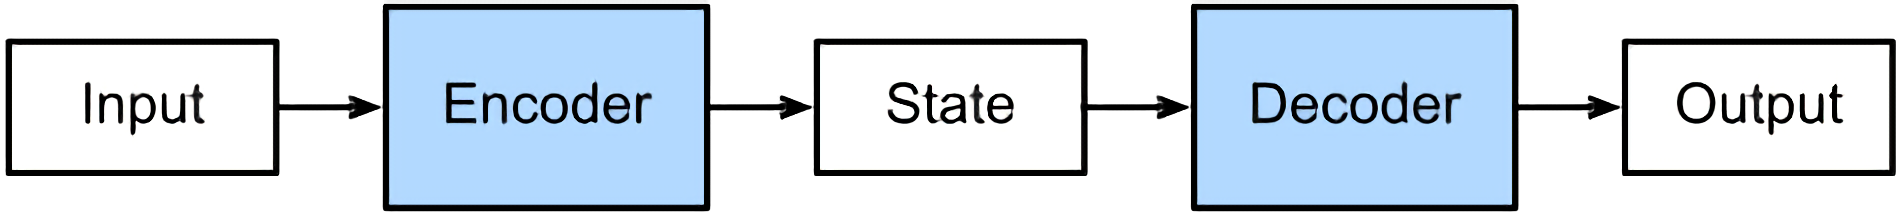
\includegraphics[width=\textwidth]{res/encoder-decoder.png}
    \caption{The encoder-decoder architecture \cite{zhang_dive_2019}.}
    \label{fig:encoder_decoder}
\end{figure}

Extraction of features at multiple scales is also important for dense prediction - a car in the distance will be differently sized to a car in the foreground, but both should be labelled accurately. This can be addressed by feeding in and parsing inputs at multiple scales, as in RefineNet \cite{lin_refinenet_2016} or using multi-scale pooling techniques, such as Spacial Pyramid Pooling (SPP) \cite{he_spatial_2014}.

Today, the DeepLab series of models is considered a benchmark for performant segmentation CNNs. DeepLab \cite{chen_semantic_2016} introduced the atrous convolution for dense prediction tasks. Atrous convolutions introduce gaps between the weights used to inform the next layer’s pixels, allowing for a larger receptive field without significantly increasing model parameters. DeepLabV2 \cite{chen_deeplab_2017} builds on this via Atrous Spatial Pyramid Pooling (ASPP), which combines PSPNet’s \cite{zhao_pyramid_2017} multi-scale features with a wider receptive field (figure ~\ref{fig:deeplab_aspp}). DeeplabV3 \cite{chen_rethinking_2017} introduces a deeper architecture and adds a resizing component to ASPP that better suits atrous convolution’s large receptive field. DeepLabV3+ \cite{chen_encoder-decoder_2018} introduced an encoder-decoder design with DeepLabV3 as the encoder, and applies a simple decoder to better refine class boundaries. DeeplabV3+ achieves 82.1\% mIoU on the Cityscapes dataset \cite{cordts_cityscapes_2016}, a common benchmark for segmentation models.

\subsection{Fast semantic segmentation}
The density and number of predictions (typically one per input pixel) required for semantic segmentation makes it one of the most computationally expensive computer vision tasks. The large number of predictions in the output layer itself is computationally expensive, but dense predictions also typically require a higher-resolution feature map, further increasing memory and compute requirements. Many state-of-the-art segmentation models are therefore only capable of running at a speed of 2-3 predictions a second on modern hardware \cite{zhao_icnet_2018}. Since many uses of segmentation, such as self-driving cars and robotics, require segmentation to be performed in real-time, extensive research has been done to improve the efficiency of semantic segmentation.

ENet (Efficient Net) \cite{paszke_enet_2016} was one of the first models to explore low-resource segmentation, focusing on reasonable accuracy capable of running in real-time on mobile devices. It achieves this by making select sacrifices to minimise model parameters and computations while mitigating drops in accuracy. Input features are quickly downsampled to a low resolution ($\frac{1}{8}$th input) with a small number of features, as minimising information density early in the model (forcing the model to “compress” image information) was found to only minimally reduce performance. The model also minimises the size of the decoder, and employs atrous and factorised convolutions to increase receptive field without increasing computation. E-Net achieves 58.3\% mIoU on the Cityscapes test set with 0.37M parameters, compared to the then state-of-the art DeepLab’s 63.1\% mIoU with 134.3M parameters.

ICNet (Image Cascade Network) \cite{zhao_icnet_2018} in 2018 was the next major model to tackle the fast segmentation problem. Initial approaches had an inherent trade-off: reduced input size increases speed, as less convolutions must be performed, but reduces segmentation accuracy, as there are less fine details. ICNet addresses this by taking in the same input image at different scales. High-resolution inputs are parsed through low-filter-count layers that are lightweight but still capable of extracting low-level details like edge and texture. Low-resolution inputs are parsed through more expensive high-filter-count layers capable of extracting high-level object information (e.g. “these pixels represent a car”), where the low resolution keeps computation time low. The computed features are then fused together through multiple “cascades” to produce the final features. This approach - delegating high-resolution branches to low-level details and vice versa - has become a staple of fast segmentation. BiSeNet \cite{yu_bisenet_2018} extends ICNet’s multi-resolution approach, finding that two ‘branches’, one high-resolution (the “spatial path”) and one low resolution (the “context path”) is most effective.

Many efficient segmentation models rely on innovations from other computer vision domains. The MobileNet \cite{howard_mobilenets_2017} classification models introduced the depthwise separable convolution block, which splits a standard convolution into a (far less expensive) combination of pointwise and depthwise convolution with minimal accuracy loss. MobileNetV2 \cite{sandler_mobilenetv2_2019} introduces the bottleneck residual block, which performs efficient convolutions by transforming inputs into a high-dimensional manifold. ContextNet \cite{poudel_contextnet_2018} uses a two-branch architecture like BiSeNet \cite{yu_bisenet_2018}, and introduces depthwise separable convolutions and bottleneck residual blocks for the high (shallow) and low (deep) resolution branches respectively. ContextNet’s successor, Fast-SCNN \cite{poudel_fast-scnn_2019}, has become a benchmark for fast segmentation performance. Fast-SCNN replaces the high-resolution branch with a “learning-to-downsample” module that downsamples the input, learns simple high-resolution features, and is used as input to the deep branch. The shallow high-resolution information is then simply fed into the final output features via a skip-connection (figure ~\ref{fig:fastscnn_architecture})

\begin{figure}[h]
    \centering
    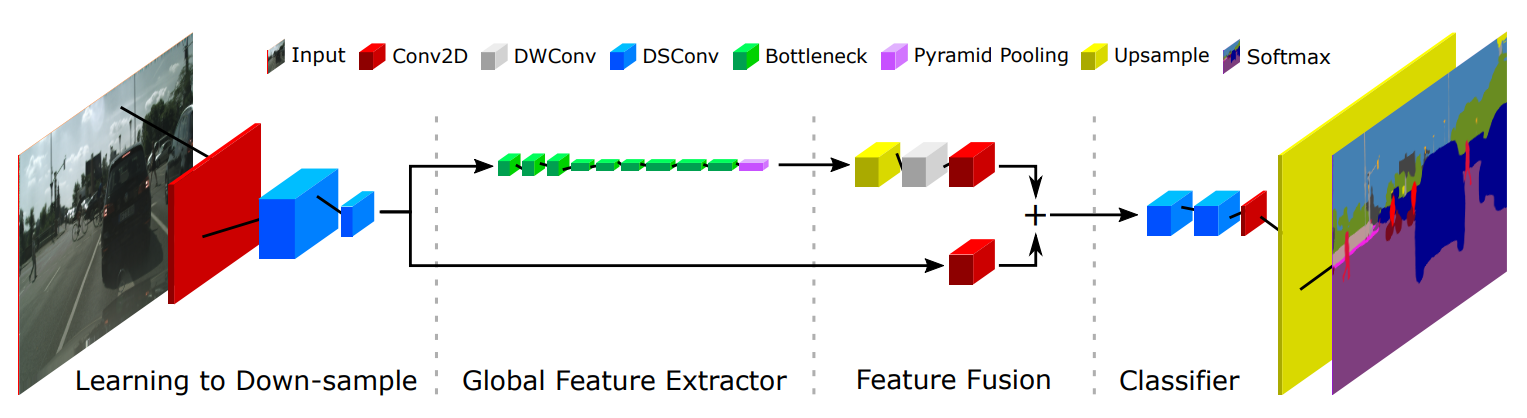
\includegraphics[width=\textwidth]{res/fastscnn-architecture.png}
    \caption{Fast-SCNN architecture \cite{poudel_fast-scnn_2019}.}
    \label{fig:fastscnn_architecture}
\end{figure}

\subsection{Transformers for semantic segmentation}

The transformer architecture revolutionised the deep learning field in 2017 \cite{vaswani_attention_2017}. Initially applied for sequence-based natural language processing (NLP) tasks, transformers propose a fundamentally different approach to CNNs. Transformers are based on the concepts of self-attention and multi-head attention. These respectively give the model the ability to determine importance between different components o fa sequence, and compute this importance in a number of different ways, simila to having multiple filters for different features in CNNs. ViT \cite{dosovitskiy_image_2021} was the first attempt to produce a fully transformer-based vision architecture (as in \cite{vaswani_attention_2017}) modified for image inputs. Rather than encoding each pixel into an input sequence (which would be prohibitively expensive), ViT groups the input image into $16 \times 16$ patches for encoding into the input sequence. Transformers became ubiquitous in NLP due to their ability to map long-distance relationships and their extreme scalability with increasing amounts of data \cite{devlin_bert_2019} \cite{radford_language_2019}. However, transformers lack the translational equivariance and locality that are believed to make CNNs so effective for vision, and experiments indeed showed that ViT is outperformed by state-of-the-art CNNs when trained on smaller datasets. However, when trained on extremely large datasets, the scalability of transformers appears to win out against these biases.

\begin{figure}[h]
    \centering
    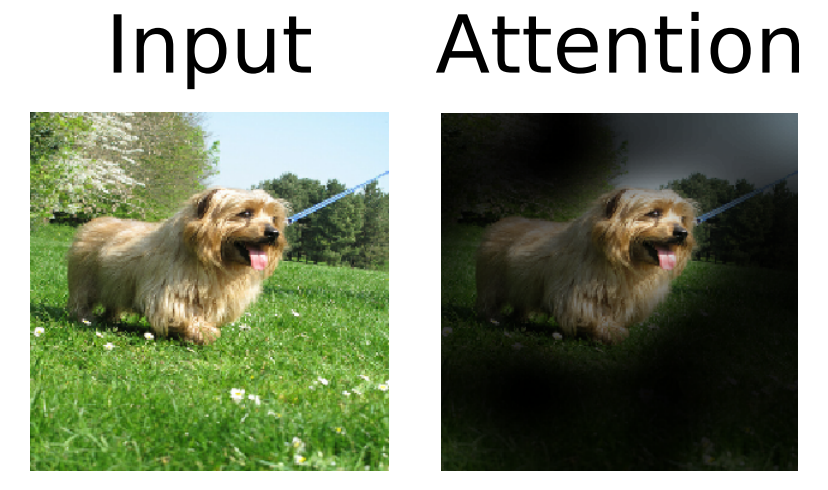
\includegraphics[scale=0.5]{res/vit-attention.png}
    \caption{Visualisation of self-attention for images in ViT \cite{dosovitskiy_image_2021}. Brighter pixels had greater importances computed between them by the transformer.}
    \label{fig:vit_attention}
\end{figure}

Other models have since built on ViT. Most significantly for segmentation, Pyramid Vision Transformer (PVT) \cite{wang_pyramid_2021} modifiers ViT to be more suitable for dense prediction, implementing $4 \times 4$ instead of $16 \times 16$ image patches for increased feature detail. To maintain performance (and develop multi-scale features), it then progressively merges patches between transformer blocks. DeIT \cite{touvron_training_2021} proposes a student-teacher and distilled training approach that allows ViT’s architecture to perform strongly even when pre-trained on far smaller datasets. Swin Transformer \cite{liu_swin_2021} builds hierarchical feature maps like PVT by merging image patches, but only computes self-attention within each window for efficiency. Twins \cite{chu_twins_2021} combines locally-grouped and global self-attention to achieve state-of-the-art performance. SETR \cite{zheng_rethinking_2021} uses an encoder-decoder architecture with a pretrained vision transformer (such as ViT or DeIT) as a backbone, and found pre-training was essential. Without pre-training, SETR achieved only 42\% mIoU on Cityscapes, worse than models with 1\% the parameters \cite{paszke_enet_2016}. However, with pre-training, SETR achieved a state-of-the-art 82.15\% mIoU on Cityscapes.

SETR demonstrated the capacity of transformers in segmentation, but was limited by its use of a backbone designed for classification. SegFormer \cite{xie_segformer_2021} addressed a number of these issues using it’s Mix Transformer Encoder (MiT). First, dense $4 \times 4$ pixel patches and progressive patch merging are used as in PVT \cite{wang_pyramid_2021}. Rather than pure-MLP layers after each attention block, SegFormer employs MLPs mixed with $3 \times 3$ convolutions without zero-padding. This leaks spatial spatial information to the model that bypasses the need for positional encoding. Combined with a simple all-MLP encoder, possible due to the transformer’s receptive field, SegFormer achieves a state-of-the art 51.0\% mIoU on the new, challenging ADE20K dataset \cite{zhou_semantic_2018}.

\begin{figure}[t]
    \centering
    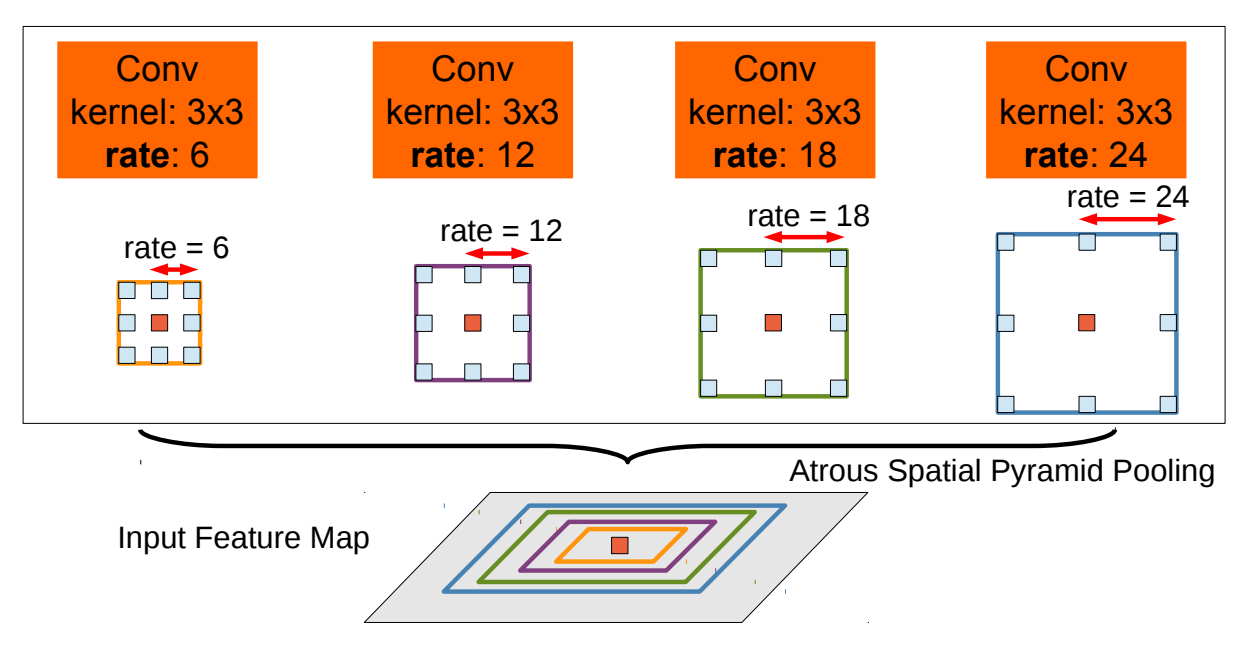
\includegraphics[scale=0.5]{res/deeplab-aspp.png}
    \caption{Visualisation of atrous spatial pyramid pooling \cite{chen_deeplab_2017}.}
    \label{fig:deeplab_aspp}
\end{figure}

\section{Significance}

% - Smaller models better for the environment and for users
% - Domain adaptation makes use of neural networks easier for everyone, including disadvantaged groups who do not possess localised training areas

\section{Innovation}

\section{Thesis Statement}

% ------------------------------------------------------------------------------
% Crack Segmentation
% ------------------------------------------------------------------------------
\chapter{Crack Segmentation}

\section{Background}
% \subsection{Semantic Segmentation}
\subsection{Crack Detection and Segmentation}
Crack detection has been a growing research area in recent years \cite{hamishebahar_comprehensive_2022}. The detection of surface-level cracks is significant in evaluating the health of structures, and achievable using automated camera-based approaches with modern computer vision techniques. Zhang \textit{et al.} \cite{zhang_road_2016}, for instance, proposed an early CNN for performing crack detection on a dataset of 500 crack images. While approaches initially focused on object detection and classification, many recent studies apply semantic segmentation \cite{hamishebahar_comprehensive_2022} due to the valuable additional information on crack shape and size it provides. Initial approaches often applied existing segmentation networks or backbones to crack detection, such as U-Net \cite{david_jenkins_deep_2018} and SegNet \cite{chen_pavement_2020}.

There are two unique issues in crack segmentation compared to other segmentation tasks. First, the thin and fine-grained nature of cracks means especially dense features must be maintained throughout the model, as any reduction in feature resolution will cause major inaccuracies in fine crack shapes. Secondly, cracks typically make up a minority of a given input image even when they are present ($<5\%$ of pixels), resulting in class imbalance. DeepCrack \cite{liu_deepcrack_2019} computes multi-scale features to ensure large and thin cracks are accurately segmented and applies a class-balanced loss computed multiple times throughout the network to address class imbalance. FPHBN \cite{yang_feature_2019} instead derives multi-scale information via a feature pyramid, and compares their approach with other models across multiple datasets. MR-CrackNet \cite{nayyeri_multi-resolution_2021} applies a modified ResNet \cite{he_deep_2015} backbone, addressing the maintaining of feature resolution by upsampling extracted features after each block.
Many of the above approaches are evaluated on unique datasets not publicly available, making comparisons challenging. A number of public datasets have been proposed for crack segmentation, including CrackBgData \cite{nayyeri_multi-resolution_2021}, CRACK500 \cite{yang_feature_2019}, and others \cite{eisenbach_how_2017} \cite{shi_automatic_2016} \cite{amhaz_automatic_2016} \cite{zou_cracktree_2012}.

\begin{figure}
    \centering
    \begin{subfigure}{.5\textwidth}
        \centering
        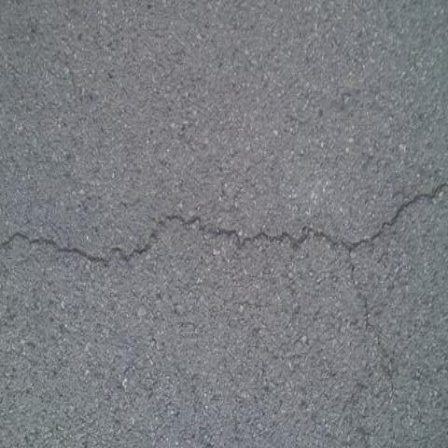
\includegraphics[width=0.8\linewidth]{res/dataset_CFD_029.png}
        \caption{Original crack image}
        \label{fig:crack-percentages-sub1}
    \end{subfigure}%
    \begin{subfigure}{.5\textwidth}
        \centering
        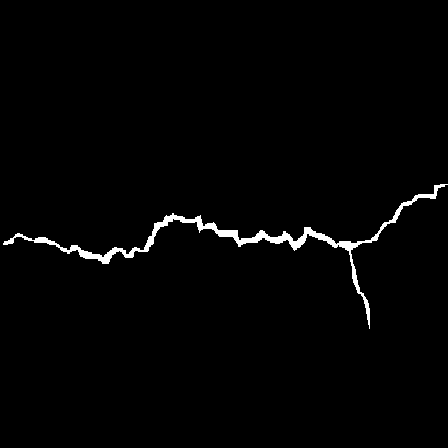
\includegraphics[width=0.8\linewidth]{res/dataset_CFD_029_label.png}
        \caption{Crack label}
        \label{fig:crack-percentages-sub2}
    \end{subfigure}
    \caption{Crack image and corresponding segmentation mask from the CFD dataset \cite{shi_automatic_2016}. Note the white `crack' class only makes up $\sim 1.5\%$ of pixels in the mask.}
    \label{fig:crack-percentages}
\end{figure}

\subsection{Efficient Crack Segmentation}
Processing efficiency is important when performing infrastructure crack detection due the large amount of images that must be processed when applied at scale. Various studies \cite{kerle_uav-based_2020} \cite{kang_autonomous_2018} have investigated the use of UAVs (Unmanned Aerial Vehicles) for high-speed crack segmentation, a system only viable with a highly efficient neural network such as Faster R-CNN \cite{ali_real-time_2021}. Recent studies have investigated efficient crack detection. SDDNet \cite{choi_sddnet_2019} maintains high-resolution features using a simple skip connection, and utilises depthwise separable convolutions and modified atrous spatial pyramid pooling techniques as introduced in the MobileNets \cite{howard_mobilenets_2017} and DeepLabV3+ \cite{chen_rethinking_2017} respectively. STRNet \cite{kang_efficient_2021} applies multi-head attention to the crack detection task, as well as a squeeze and excitation method for maintaining high feature detail.
These approaches are similar to traditional efficient segmentation architectures in the maintaining of different architectural components focusing on low and high-level features, but typically with a particular focus on high-resolution feature maps for the fine-grained crack segmentation task.

\section{The SC-CrackSeg Model}

% Talk about:
% - The idea behind crackseg (basically the introduction)
% - The dataset we used
% - How it was based on our previous papers
% - How it performed (maybe put a little table)

% - End with that there were still a number of things to explore regarding the model

The use of a separate branch for maintaining high-resolution features in crack segmentation models \cite{nayyeri_multi-resolution_2021} is similar to the deep-brach/shallow-branch approach used in efficient segmentation models \cite{yu_bisenet_2018} \cite{poudel_contextnet_2018}. This key realisation is what lead to the development of our model, SC-CrackSeg, which sought to apply a proven architectural paradigm achieve lightweight, efficiency, and performant crack segmentation. We used our team's previous model, SCMNet \cite{singha_scmnet_2021}, as a baseline. In SCMNet, deep (low-resolution) and shallow (high-resolution) features are repeatedly merged and feature-extracted before being fed back into their respective branches, maintaining both global and local features while permitting both to learn from one another. We posit applying this approach to crack segmentation would allow for the efficient learning of global and high-resolution crack features while retaining the computational efficiency such approaches often struggle to achieve.

% THESE GO SOMEWHERE:
% - Due to the small number of images available in each dataset, our approach applies a merged combination of images from multiple datasets for training.
The key realisation we made was that that the use of a separate branch for maintaining high-resolution features in crack segmentation models \cite{nayyeri_multi-resolution_2021} is similar to the deep-brach/shallow-branch approach used in efficient segmentation models \cite{yu_bisenet_2018} \cite{poudel_contextnet_2018}. This is what lead to the development of our model, SC-CrackSeg, with which we hoped to use a proven architectural paradigm to apply the efficiency and performance of lightweight segmentation models to the crack segmentation task. Particularly, we focused on our team's previous model, SCMNet \cite{singha_scmnet_2021}. In SCMNet, deep (low-resolution) and shallow (high-resolution) features are repeatedly merged and feature-extracted before being fed back into their respective branches, maintaining both global and local features while permitting both to learn from one another. We posit applying this approach to the crack segmentation task would allow for the efficient learning of high-resolution crack features while retaining the computational efficiency such approaches often struggle to achieve.

We made a number of changes to SCMNet to better suit it to the crack segmentation task and generally improve it. We move from a two-input model to a single-input model to improve efficiency and simplicity of implementation. We modify SCMNet's Context Mining Module (CMM) by eliminating its image pooling components which contribute to boundary degeneration - especially significant with crack segmentation's fine boundaries and shapes. We also deploy a simplified feature fusion module, inspired by BiSeNet \cite{yu_bisenet_2018}, to aggregate the final features extracted from the two branches. % TODO go over additions in detail

\subsection{Datasets}
Another key innovation of the paper was the use of a unified dataset to evaluate SC-CrackSeg's performance. As many datasets used to train and evaluate other crack segmentation models are either small or not publicly available, we use a combined dataset of 12 different source crack segmentation datasets, all using the same labelling scheme. Retrieved from Kaggle \footnote{\url{https://www.kaggle.com/datasets/lakshaymiddha/crack-segmentation-dataset}}, this dataset provided us with 9505 train and 1695 test images. While unorthodox, we find this dataset to be exceptionally challenging due to the large variety of image types it contains, from extremely thick to extremely thin cracks, different surfaces, and even samples that contain NO cracks at all (which can be considered testing for false positives). We identify and amend a number of issues in this dataset, and then use it to benchmark a number of existing state-of-the art crack segmentation approaches against SC-CrackSeg.

\subsection{Class Imbalance}
Besides feature resolution, class imbalance is the other key domain-specific issue in crack segmentation \cite{hamishebahar_comprehensive_2022}. Due to the overwhelming majority of "no crack" classes, the model is implicitly encouraged to prioritise predicting them in each pixel. Therefore, models must often be encouraged to accurately predict the minority class through class balancing. This is most commonly done by simply weighting the produced model losses depending on the sample, with less common samples receiving higher weights. In semantic segmentation, where each pixel in an image effectively contains it's own loss, we achieved this by using the ground truth to map a multiplication operation onto the per-pixel losses. The weights chosen for each class can vary, but the inverse of each classes proportion in the training dataset is typically used \cite{kochkarev_data_2020}.

\hspace*{4mm}
\begin{lstlisting}[language=Python, caption=Weighted categorical crossentropy function in python using TensorFlow 2.1]
def weighted_cat_crossentropy(target, output, class_weights, axis=-1):
    # scale preds so that the class probas of each sample sum to 1
    output = output / math_ops.reduce_sum(output, axis, True)

    epsilon_ = _constant_to_tensor(epsilon(), output.dtype.base_dtype)
    output = clip_ops.clip_by_value(output, epsilon_, 1. - epsilon_)

    # compute per-pixel categorical losses
    cat_losses = tf.reduce_sum(target * math_ops.log(output), axis=axis)
    
    # Apply class weights
    weight_indices = tf.argmax(target, axis=-1)
    weight_map = tf.gather(class_weights, indices=weight_indices)
    weighted_cat_losses = cat_losses * weight_map
    
    return - 1. * weighted_cat_losses
\end{lstlisting}

\subsection{Initial Results}
We find SC-CrackSeg's combination of efficiency and performance to be highly competitive. Typically, mean intersection over union (mIoU) is used to present segmentation results, but crack segmentation is highly unbalanced - focusing on one class (no crack) would skew model results. Therefore, we also assess using F1 score to better consider false positives and false negatives across classes. In terms of pure performance, SC-CrackSeg is slightly beaten by other models like DeepCrack (\autoref{tab:sc-crackseg-initial-performance-comparison}). DeepCrack achieves 77.23\% mIoU and 85.49\% mean F1 score, while SC-CrackSeg produces 77.0477\% mIoU and 85.34\% mean F1. However, SC-CrackSeg is far more efficient (\autoref{tab:sc-crackseg-initial-efficiency-comparison}). SC-CrackSeg is over 12 times smaller and 4 times faster than DeepCrack. DeepCrack possesses 14.7 million parameters (size of weights) and requires 78.8GFlops of computation per prediction, while SC-CrackSeg requires only 1.24 million parameters and 2.8 GFlops. When optimised for performance using Nvidia's TensorRT, SC-CrackSeg achieves a speed of 220 predictions per second.


\begin{table*}[ht]
    \begin{adjustbox}{width=\columnwidth,center}
        % \centering
        \begin{tabular}{|c|c|c|c|c|c|c|c|c|c|c|c|c|c|}
            \hline
                                                              &                & \multicolumn{3}{|c|}{\textbf{IoU}} & \multicolumn{3}{|c|}{\textbf{F1 score}} & \multicolumn{3}{|c|}{\textbf{Precision}} & \multicolumn{3}{|c|}{\textbf{Recall}}                                                                                                      \\
            \hline
            {Model}                               u           & {Accuracy}     & {BG}                               & {Crack}                                 & {mIoU}                                   & {BG}                                  & {Crack} & {mF1}          & {BG}    & {Crack} & {aP}           & {BG}    & {Crack} & {aR}           \\
            \hline
            {DeepLab \cite{chen_encoder-decoder_2018}}        & {98.43}        & {98.50}                            & {52.28}                                 & {75.39}                                  & {99.24}                               & {68.66} & {83.95}        & {98.97} & {79.25} & {89.11}        & {99.52} & {60.57} & {80.05}        \\
            \hline
            {U-Net \cite{}}                                   & {98.18}        & {98.2}                             & {48.97}                                 & {73.58}                                  & {99.09}                               & {65.74} & {82.42}        & {98.96} & {70.62} & {84.79}        & {99.23} & {61.49} & {80.20}        \\
            \hline
            {SegNet\cite{chen_pavement_2020}}                 & {98.27}        & {98.30}                            & {52.17}                                 & {75.23}                                  & {99.14}                               & {68.57} & {83.85}        & {99.09} & {71.15} & {85.12}        & {99.19} & {66.17} & {82.63}        \\
            \hline
            {DeepCrack\cite{liu_deepcrack_2019}}              & \textbf{98.52} & {98.57}                            & {55.89}                                 & \textbf{77.23}                           & {99.28}                               & {71.70} & \textbf{85.49} & {99.13} & {77.95} & {84.54}        & {99.44} & {66.38} & \textbf{82.91} \\
            \hline
            {MR-CrackNet\cite{nayyeri_multi-resolution_2021}} & {97.88}        & {97.19}                            & {47.69}                                 & {72.80}                                  & {98.95}                               & {64.58} & {81.76}        & {99.11} & {62.59} & {80.85}        & {98.79} & {66.71} & {82.70}        \\
            \hline
            {SCMNet\cite{singha_scmnet_2021}}                 & {98.39}        & {98.41}                            & {51.33}                                 & {74.87}                                  & {99.20}                               & {67.84} & {83.52}        & {98.91} & {77.51} & {88.21}        & {99.48} & {60.32} & {79.30}        \\
            \hline
            {SC-CrackSeg}                                     & \textbf{98.52} & {98.52}                            & {55.55}                                 & {77.04}                                  & {99.25}                               & {71.43} & {85.34}        & {99.05} & {78.14} & \textbf{88.59} & {99.46} & {65.78} & {82.32}        \\
            \hline
            \multicolumn{11}{l}{}
        \end{tabular}
    \end{adjustbox}
    \caption{Performance evaluation of different models on crack test set}%\label{tab5}
    \label{tab:sc-crackseg-initial-performance-comparison}
\end{table*}

\begin{table*}
    \begin{adjustbox}{width=\columnwidth,center}
        \centering
        \begin{tabular}{|c|c|c|c|c|c|c|c|c|c|}
            \hline
            {}            & {}           & {}           & \multicolumn{5}{|c|}{\textbf{FPS of different types of model}} & {}          & {}                                                                                                                    \\
            \hline
            {Model}       & {Param.(M)}  & {GFLOPs}     & {Keras}                                                        & {TF}        & {TF-TRT32}   & {TF-TRT16}   & {TRT-INT8}   & {\begin{tabular}{@{}c@{}}Training\\time(s)\end{tabular}} &
            {\begin{tabular}{@{}c@{}}Model \\size (MB)\end{tabular}}                                                                                                                                                                                           \\
            \hline
            {DeepLab}     & {41.0}       & {78.8}       & {20}                                                           & {21}        & {32}         & {48}         & {82}         & {415}                                                    & {158}         \\
            \hline
            {U-Net}       & {31.0}       & {1740.0}     & {31}                                                           & {30}        & {39}         & {39}         & {50}         & {348}                                                    & {355}         \\
            \hline
            {SegNet}      & {29.4}       & {245.0}      & {32}                                                           & {32}        & {44}         & {45}         & {56}         & {316}                                                    & {225}         \\
            \hline
            {DeepCrack}   & {14.7}       & {123.0}      & {33}                                                           & {33}        & {48}         & {50}         & {65}         & {257}                                                    & {112}         \\
            \hline
            {MR-CrackNet} & {17.7}       & {331}        & {14}                                                           & {14}        & {25}         & {28}         & {45}         & {1013}                                                   & {203}         \\
            %\hline
            %{MR-CrackNet} & {17.7} & {331} & {} &  {} & {} & {} &  {} & {} & {}\\
            \hline
            {SCMNet}      & \textbf{1.2} & {3.3}        & {61}                                                           & {67}        & {111}        & {111}        & {114}        & {182}                                                    & {10.7}        \\
            \hline
            {SC-CrackSeg} & {1.24}       & \textbf{2.8} & \textbf{70}                                                    & \textbf{78} & \textbf{216} & \textbf{216} & \textbf{220} & \textbf{93}                                              & \textbf{10.8} \\
            \hline
            \multicolumn{10}{l}{}
        \end{tabular}
    \end{adjustbox}
    \caption{Efficiency analysis against SC-CrackSeg}
    \label{tab:sc-crackseg-initial-efficiency-comparison}
\end{table*}


\section{Further exploration of SC-CrackSeg and Competitors}
\subsection{The Performance of SDDNet}
While Tanmay Singha and I implemented a number of existing crack segmentation models for fair comparison against SC-CrackSet, some could not be completed due to time limitations. Notably, a from-scratch implementation of 2019's SDDNet \cite{choi_sddnet_2019} was in development, but could not be completed in time for the publication. The SDDNet implementation has since been completed and evaluated, and results are surprising: SDDNet, at a similar parameter count and computational efficiency, outperforms all other models tested by a significant margin.

SDDNet was introduced in 2019 as a novel design specifically targeting the low class count and large object shapes present in the crack segmentation task while focusing on efficiency. A single-branch encoder-decoder model, SDDNet utilises atrous spacial pyramid pooling and dense skip connections to extract features. Notably, it performs all of its depthwise separable convolutions in reverse, doing pointwise convolution first to initially reduce dimensionality and further reduce computation over the traditional method. While not explicitly stated, we intuit that the reduced channel resolution from performing depthwise first is not as significant in a low-class task like crack segmentation, where the feature space is semantically sparse compared to other tasks. It also removes the global average pooling component of its Atrous Spacial Pyramid Module as it was found to strongly regularise, detrimental to a low-parameter model.

\begin{figure}[ht!]
    \centering
    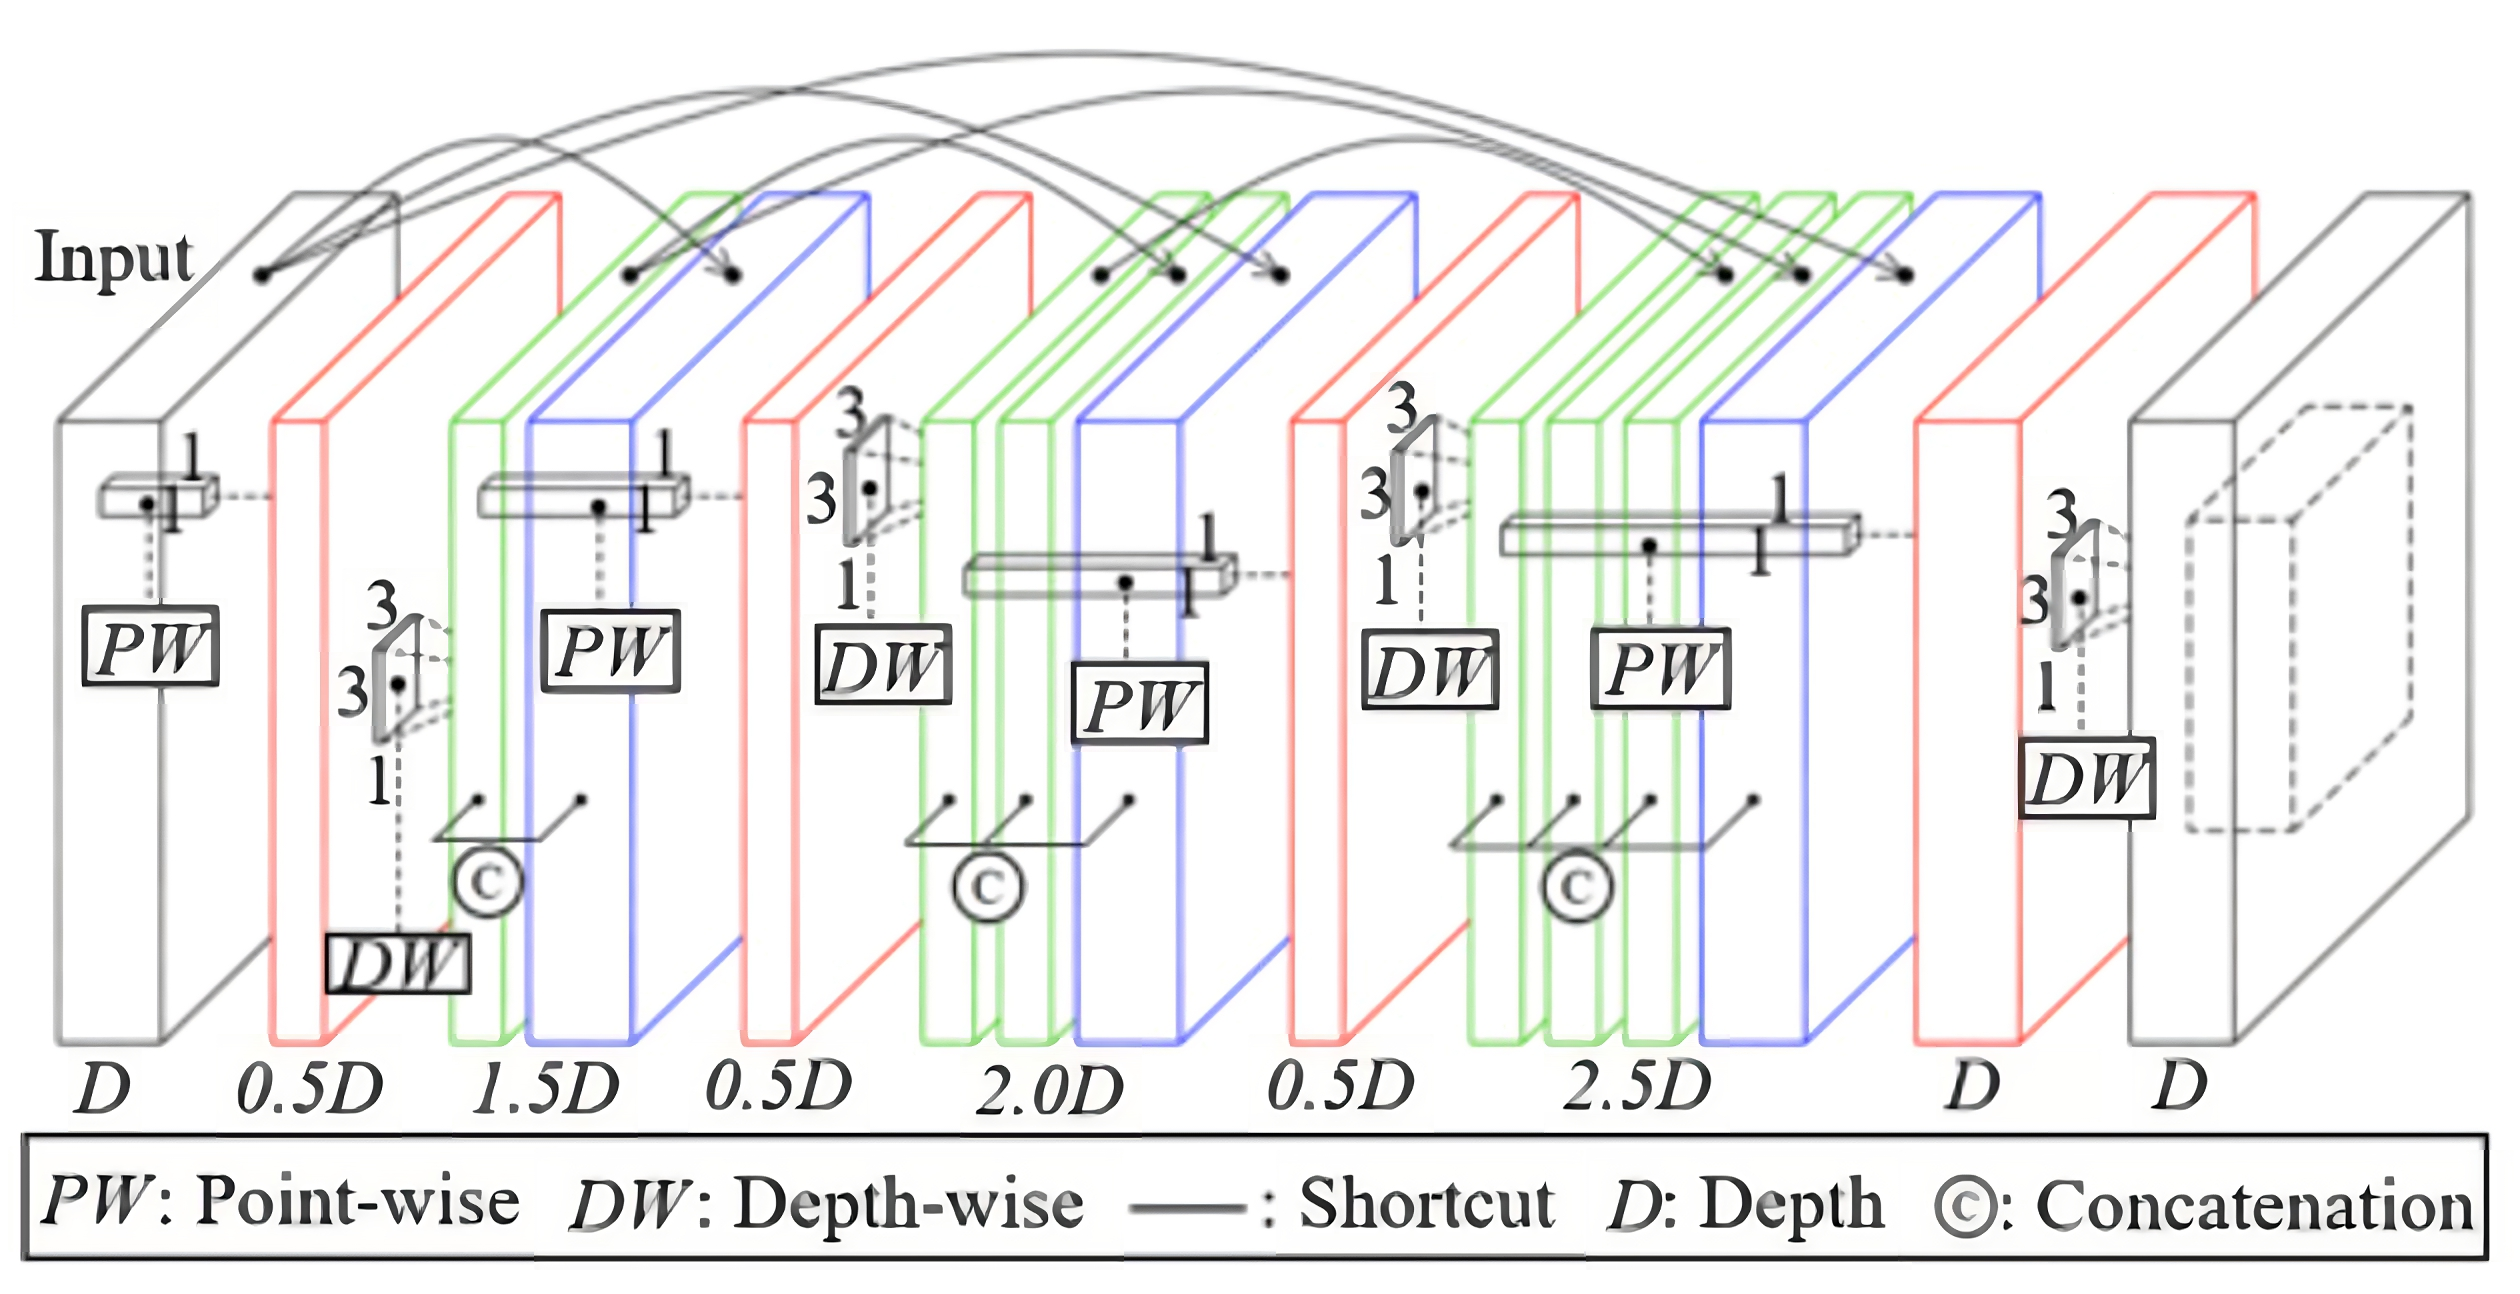
\includegraphics[width=0.5\textwidth]{res/sddnet-densep-module.png}
    \caption{SDDNet's \cite{choi_sddnet_2019} DenSep module. The number of channels maintained throughout the module is constant, though depth is periodically increased through concatenation and skip connections.}
    \label{fig:densep-module}
\end{figure}

SDDNet is primarily made up of DenSep modules, which consist of repeated reverse DSConv operations. The output of each operation is then fed into the input of all subsequent ones, permitting a large amount of feature extraction while keeping the number of channels very low, and thus computation extremely efficient. The authors found that, in terms of multiplications done, the DenSep module reduces computing cost by over 70\% an approach using traditional convolutions.

Finally, SDDNet's decoder upsamples input features in two stages, applying a skip connection from early in the model (when features were high resolution) combined with separable convolutions between the upsamples. This aids in the refinement of feature boundaries before they are upsampled further. SCMNet identified that multi-stage upsampling was, while more computationally expensive, significantly more effective than a single upsample \cite{singha_scmnet_2021}. SC-CrackSeg uses a similar approach to SDDNet, upsampling multiple times using skip connections from previous positions in the model. However, SC-CrackSeg downsamples far more than SDDNet, and only performs skip connections during the lower-resolution stages of upsampling.
% TODO add more figures, add quant analysis figures 
\subsection{Modifications to CrackSeg}

\begin{figure*}[]
    \centering
    \begin{subfigure}[b]{0.3\textwidth}
        \centering
        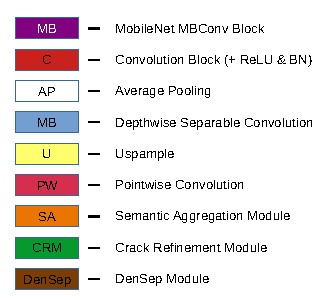
\includegraphics[width=\textwidth]{res/crack-experiment-diagrams/legend.pdf}
        \label{fig:sc-crackseg-versions-legend}
    \end{subfigure}
    \begin{subfigure}[b]{0.6964\textwidth}
        \centering
        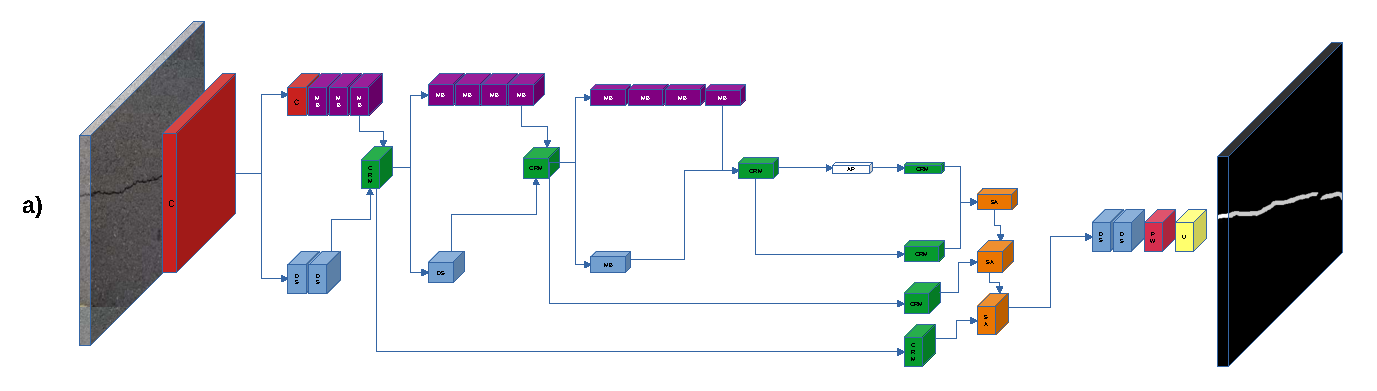
\includegraphics[width=\textwidth]{res/crack-experiment-diagrams/sc-crackseg.pdf}
        \caption{SC-CrackSeg}
        \label{fig:sc-crackseg-versions-sc-crackseg}
    \end{subfigure}
    \begin{subfigure}[b]{0.6964\textwidth}
        \centering
        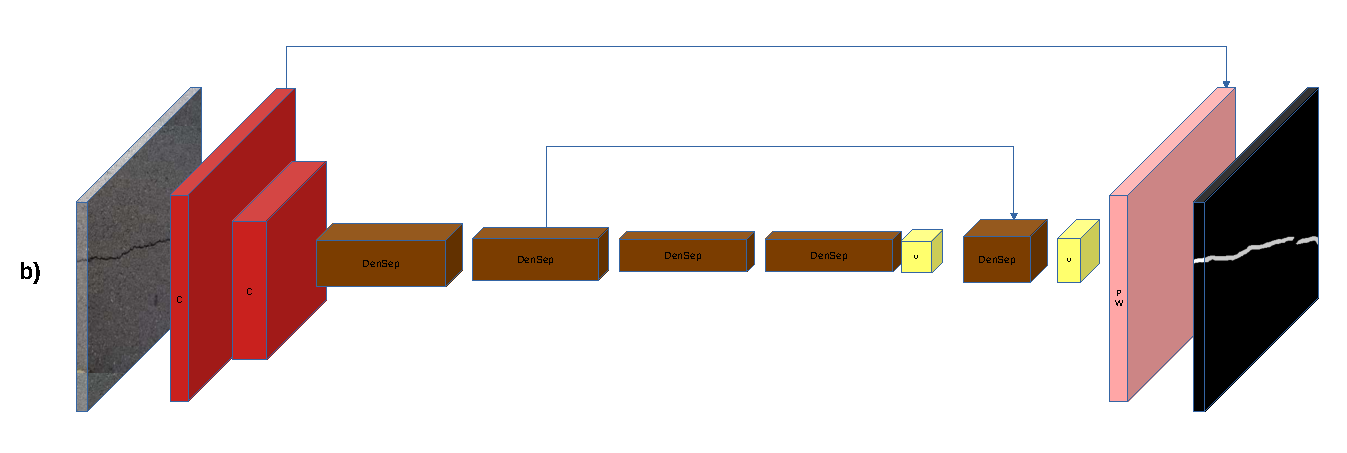
\includegraphics[width=\textwidth]{res/crack-experiment-diagrams/sddnet.pdf}
        \caption{SDDNet}
        \label{fig:sc-crackseg-versions-sddnet}
    \end{subfigure}
    \begin{subfigure}[b]{0.6964\textwidth}
        \centering
        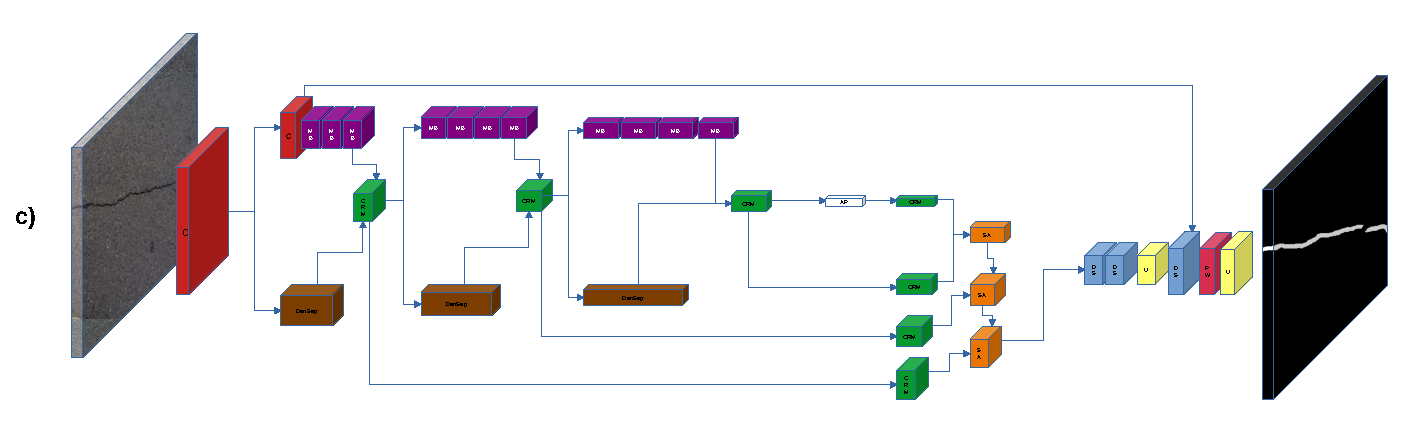
\includegraphics[width=\textwidth]{res/crack-experiment-diagrams/sc-crackseg-densep-skip.pdf}
        \caption{SC-CrackSeg with DenSep and skip connection}
        \label{fig:sc-crackseg-versions-sc-crackseg-densep-skip}
    \end{subfigure}
    \begin{subfigure}[b]{0.6964\textwidth}
        \centering
        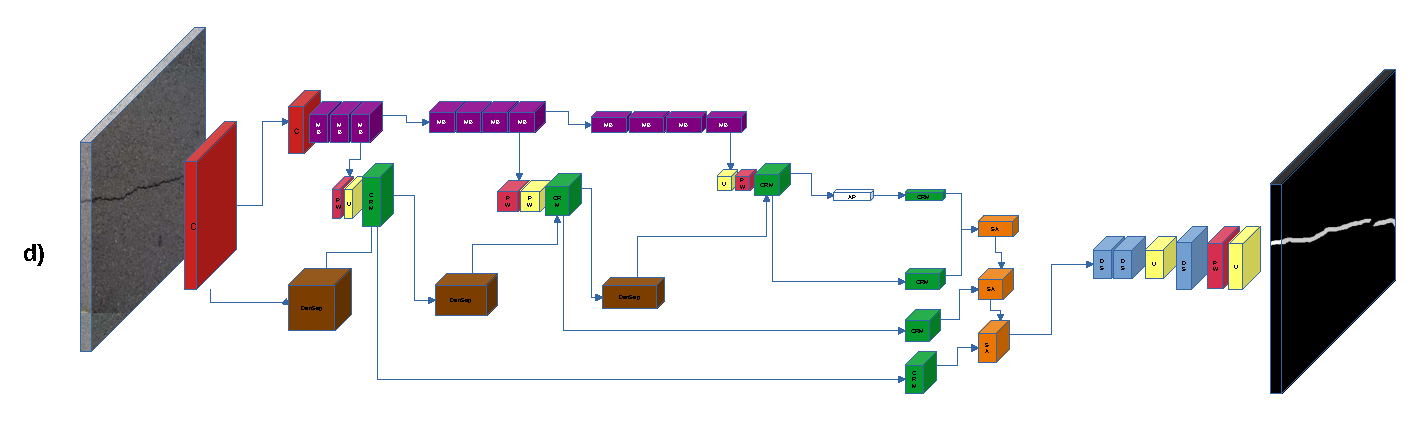
\includegraphics[width=\textwidth]{res/crack-experiment-diagrams/sc-crackseg-densep-upsample.pdf}
        \caption{SC-CrackSeg with DenSep and upsampled shallow branch}
        \label{fig:sc-crackseg-versions-sc-crackseg-densep-upsample}
    \end{subfigure}

    \caption{Diagrams representing significant architectures during experimentation.}
    \label{fig:sc-crackseg-versions}
\end{figure*}

Based on the strong performance of a simple model like SDDNet, we hypothesised that SC-CrackSeg could be optimised further towards the crack segmentation task. Therefore, we experimented with our architecture, seeking to take into consideration many of the design choices made in successful models like SDDNet.

I started my model development with a naive intuition: SC-CrackSeg's issues were caused by a lack of direct adaptation to the crack segmentation scenario - the model was too deep and too low-resolution. Two things have been identified throughout the review of crack segmentation - output quality depends on high-resolution [SOURCE], and the actual act of class distinguishing is simple relative to other tasks [SOURCE]. The intuition was that decreasing the amount of downsampling done by the model would improve the granularity of produced features, while reducing the number of channels would counteract the performance cost of this operation while only minimally affecting results as performance as less channel depth was required for the crack segmentation task in the first place. However, experiments showed the problem was not that simple. Increasing resolution immediately became prohibitively expensive in terms of performance, while decreasing channels significantly (to a maximum of 64) destroyed model performance.

Upon these initial failures, I instead explored a more nuanced approach to the intuitions. I designed iterations of SC-CrackSeg that place model's focus on the shallow branch while minimising the effect on the deep branch wherever possible. Unfortunately, I found any approach increasing shallow network convolution resolution to be unfeasible when combined with the deep branch, and also found simply increasing the number of convolutions in the shallow branch had minimal effect on model performance.

Inspired by SDDNet, I replaced all shallow branch blocks with DenSep modules (\autoref{fig:sc-crackseg-versions-sc-crackseg-densep-skip}). The concatenation-based approach to feature extraction allows feature resolution to be maintained in the deep branch (where it is most essential) while minimising the downsampling done, as DenSep modules only downsample in their final block (\autoref{fig:densep-module}). An initial model with only these changes achieved promising results. An issue, however, is that since the deep and shallow branches share information, their dimensions must periodically match at the 3 information sharing points in the model, forcing the shallow branch to be downsampled further than in SDDNet. This is likely to reduce output granularity. I first addressed this by adjusting the information sharing system. Information would only be shared from the deep to the shallow branch, and the shallow branch would downsample less and possess less channels to counteract computing costs. Information sharing could then occur by reducing the deep branch's channels via pointwise convolution and then upsampling. These combined results produced one of our final architectures (\autoref{fig:sc-crackseg-versions-sc-crackseg-densep-upsample}).

Another consideration was the significance of the gradual upsampling skip connection in SDDNet. While SC-CrackSeg already possesses a number of skip-like connections and gradual upsampling, these largely occur to increase from lower resolutions, and are still followed by an $8 \times$ upsample. Therefore, we added another skip connection with the early parts of the model before final output is computed. The skip connection features were initially resolved with the decoder features using another SA module as with the other skip connections in the model, but we found this to degrade performance (perhaps as the SA module failed to produce fine output at the highest resolutions). Replacing the SA module with a simple depthwise separable convolution resolved these issues. This approach was most successful, and while multiple variations were assessed, any increase in complexity (introducing upsamples or adding further skip connections) seemed to decrease model stability and quickly cause overfitting issues. Even so, our final model outperforms SDDNet in assessment while possessing a significantly lower number of flops and parameters.% TODO CHECK WHAT I SAID ABOUT THE SA MODULE BEING BAD HERE % ALSO CHECK THAT PARAMETERS ARE ACTUALLY LOWER

% ALSO ADD we were able to get fine crack details (the little gap) that none of the previous models could

% PARAMETERS ETC COMPARISON TABLE HERE

Even though our best approaches introduced SDDNet's DenSep module, we notably did not borrow another core feature - the final ASPP stage. This is as SC-CrackSeg already possesses high-quality global context refinement via its depp branch, which aggregates global context through repeated downsampling and then merges these with the more fine features.

\subsection{Experimental Setup}
All new experiments were run using using my available experimental environment, which consisted of a single Nvidia RTX 2080Ti, running Tensorflow 2.1 and python 3.6 using the Nvidia TensorFlow Docker container (nvcr.io/nvidia/tensorflow:20.03-tf2-py3). All experiments used the same random seed for consistency.

\subsection{Experiment Results}

% TODO add figure showing class-imbalanced predictions

Only some of the above experimental models were assessed. All models were trained to 300 epochs on the custom combined crack dataset.

For brevity, the following terms will describe SC-CrackSeg modifications:
\begin{itemize}
    \item \textbf{SC-CrackSeg-1}: Less downsampling and max channels of 64
    \item \textbf{SC-CrackSeg-2}: Less deep branch blocks, reduced channel numbers near end of encoder (specifically, remove 1 convolution block in deep block sequences and set 3rd deep branch block sequence to $108$ and $128$ channels instead of $128$ and $160$)
    \item \textbf{SC-CrackSeg-3}: Replace shallow branch blocks with DenSep module, add skip connection (\autoref{fig:sc-crackseg-versions-sc-crackseg-densep-skip})
    \item \textbf{SC-CrackSeg-4}: Replace shallow branch blocks with DenSep module, keep deep branch shallower and combine with deep branch via upsamples (\autoref{fig:sc-crackseg-versions-sc-crackseg-densep-upsample})
\end{itemize}
% TODO change SC-CrackSeg-2 prediction, results, add all ablations
\begin{table*}[htbp]
    \begin{adjustbox}{width=\columnwidth,center}
        \begin{tabular}{|p{0.2\textwidth}|c|c|c|c|c|c|c|c|}
            \hline
                                                & \textbf{U-Net} & \textbf{SDDNet} & \textbf{SC-CrackSeg} & \textbf{SCMNet} & \textbf{SC-CrackSeg-1} & \textbf{SC-CrackSeg-2} & \textbf{SC-CrackSeg-3} & \textbf{SC-CrackSeg-4} \\
            \hline
            \textbf{Parameters}                 & 0.35M          & \textbf{0.33M}  & 1.27M                & 1.26M           & 0.63M                  & 1.01M                  & 1.51M                  & 1.3M                   \\
            \hline
            \textbf{Flops}                      & 2.44M          & 2.75M           & 1.4M                 & 1.62M           & 18.12M                 & \textbf{1.24M}         & 2.16M                  & 4.32M                  \\
            \hline
            \textbf{Crack Test Set Performance} & 0.796          & \textbf{0.815}  & 0.807                & 0.81            & 0.63                   & 0.808                  & 0.812                  & 0.803                  \\
            \hline
            \textbf{FPS}                        & \textbf{27.05} & 15.84           & 15.94                & 16.87           & 12.75                  & 15.87                  & 14.01                  & 13.15                  \\
            \hline
        \end{tabular}
    \end{adjustbox}
    \caption{Performance evaluation of modifications (and SDDNet) on Crack Test set.}%\label{tab5}
\end{table*}

SC-CrackSeg-1 achieved extremely poor results, and was highly prone to overfitting. Removing even 2 downsamples early in the model also massively increased the number of parameters, making this model too complex for the crack segmentation task and seemingly not permitting proper receptive field. SC-CrackSeg-2 was significantly more successful, removing unnecessary components of the original architecture. This model maintains the performance of the original SC-CrackSeg while possessing significantly fewer parameters and flops. SC-CrackSeg-3 achieves the strongest results out of our models, and achieves a strong balance between performance and cost. While SC-CrackSeg-4 achieved promising results, performing repeated upsamples significantly increases the model parameters. Ultimately, SDDNet achieves the strongest qualitative results, and does so with far fewer parameters than other models - a testament to the success of simple designs in the crack segmentation space. However, it possesses greater flops than our SC-CrackSeg implementations, affecting prediction time. I believe there may be some issues with the prediction time results, perhaps caused by the containerised training setup used - SC-CrackSeg-1 achieved far faster results than expected considering it has many times the flops of other models, and all models are slower than expected and highly similar in performance.

\begin{figure}[htbp]
    \begin{tabular}{ccc}
        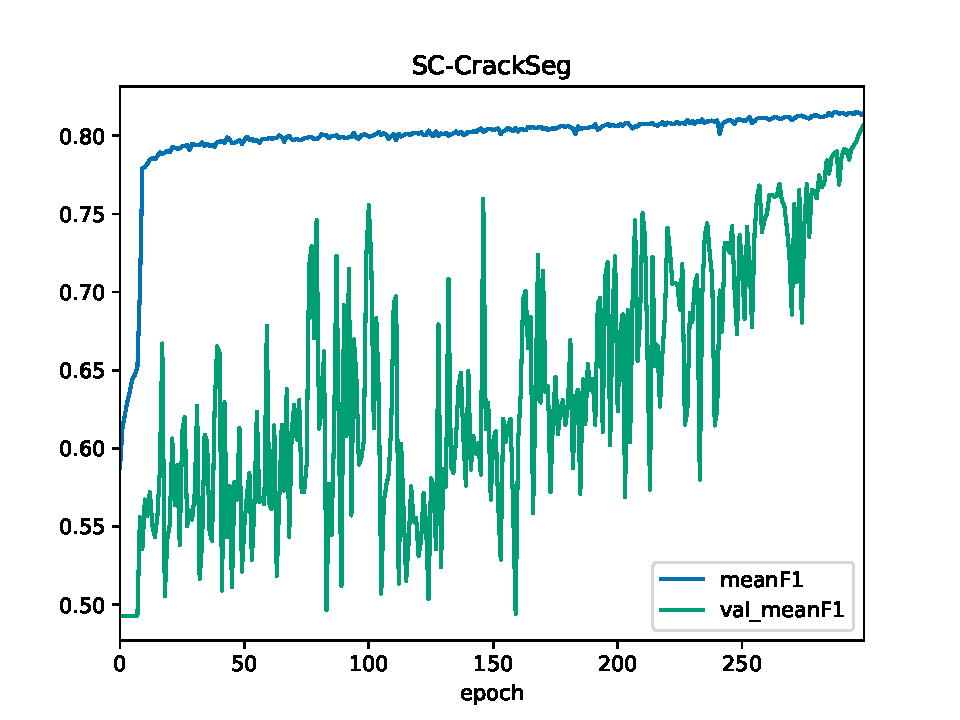
\includegraphics[width=0.3\textwidth]{res/crack-experiments-training-curves/sc-crackseg.pdf}   & 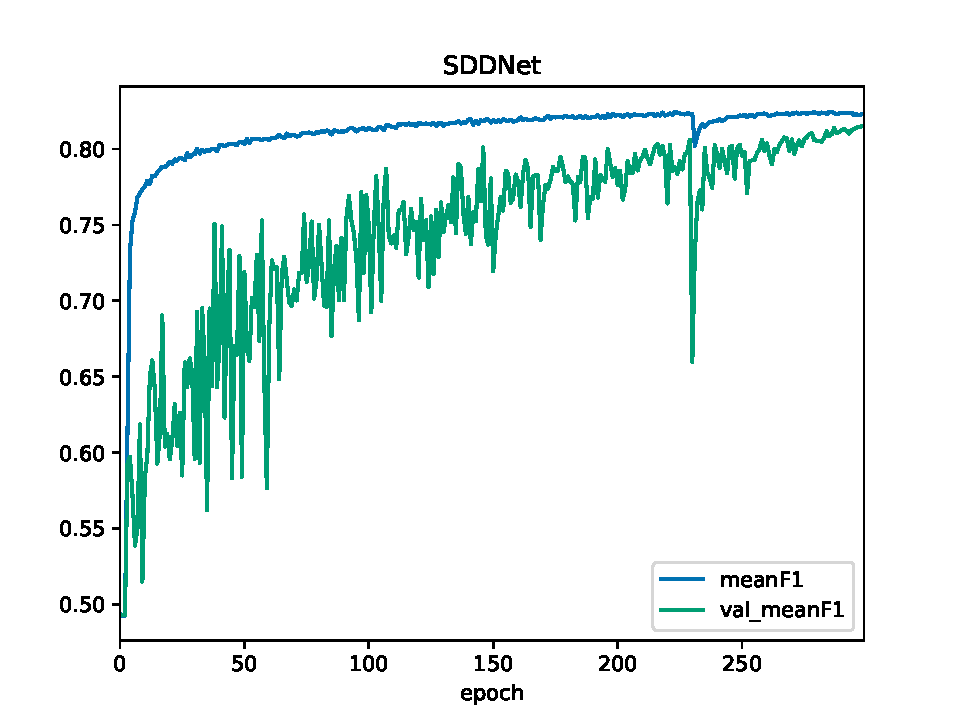
\includegraphics[width=0.3\textwidth]{res/crack-experiments-training-curves/sddnet.pdf}        & 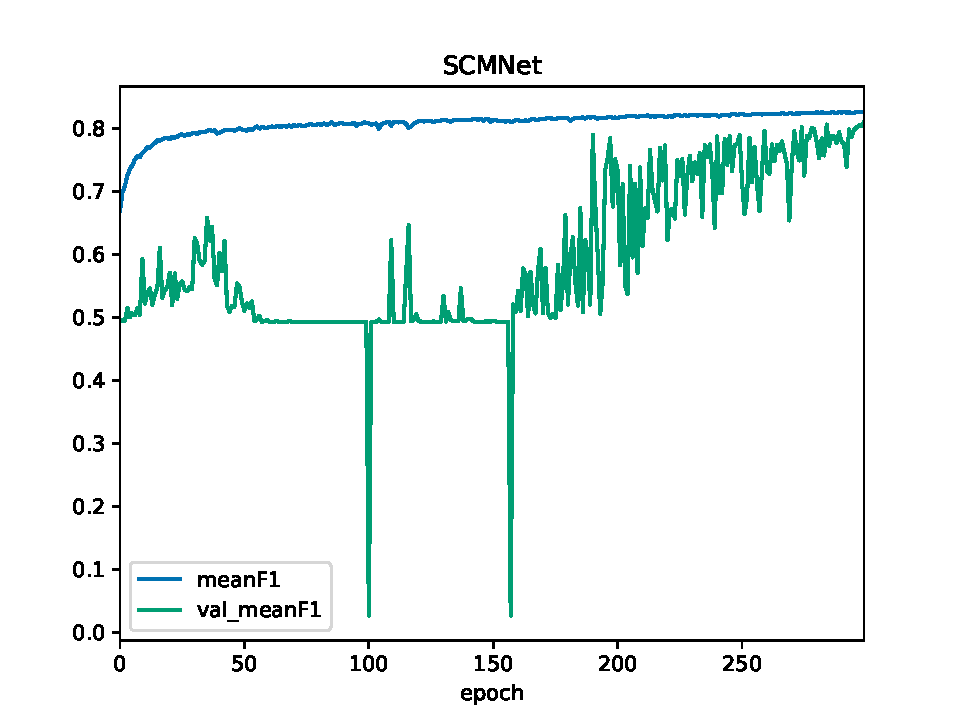
\includegraphics[width=0.3\textwidth]{res/crack-experiments-training-curves/scmnet.pdf}        \\
        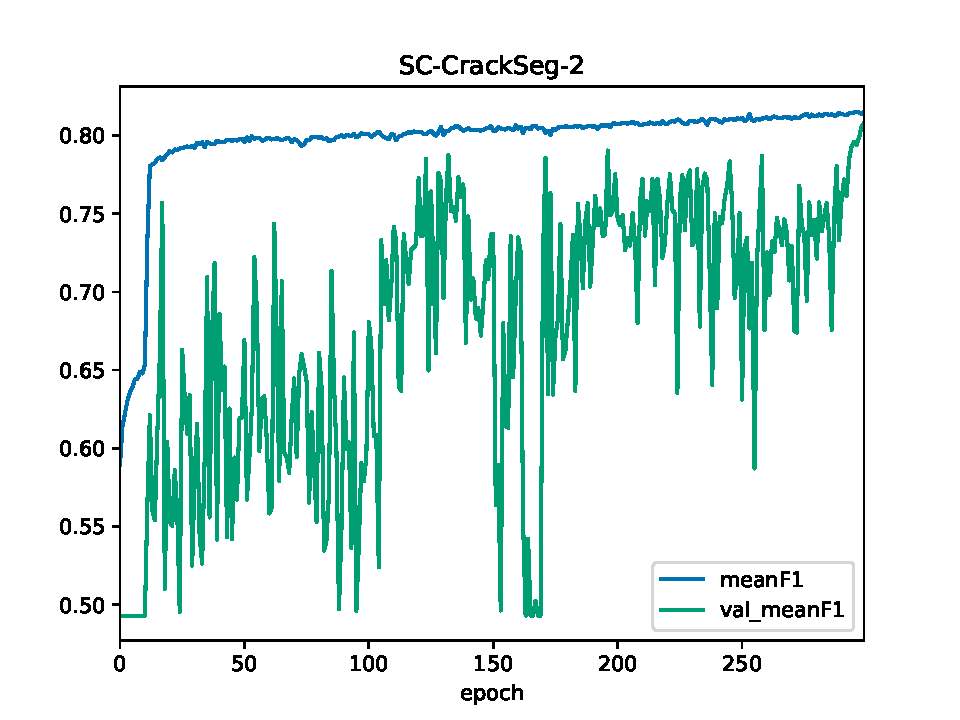
\includegraphics[width=0.3\textwidth]{res/crack-experiments-training-curves/sc-crackseg-2.pdf} & 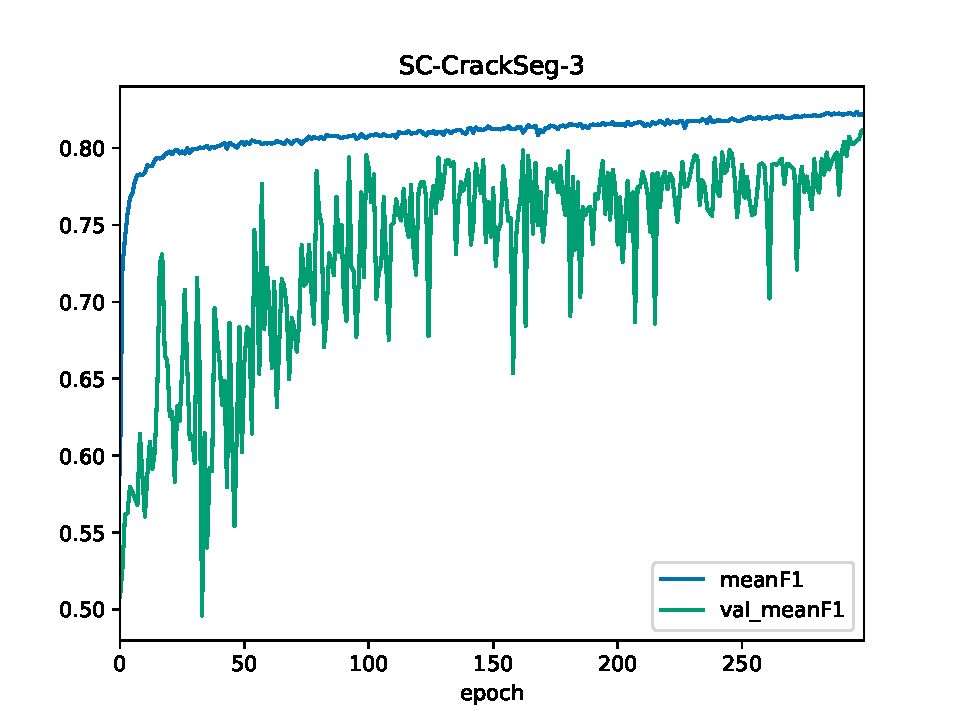
\includegraphics[width=0.3\textwidth]{res/crack-experiments-training-curves/sc-crackseg-3.pdf} & 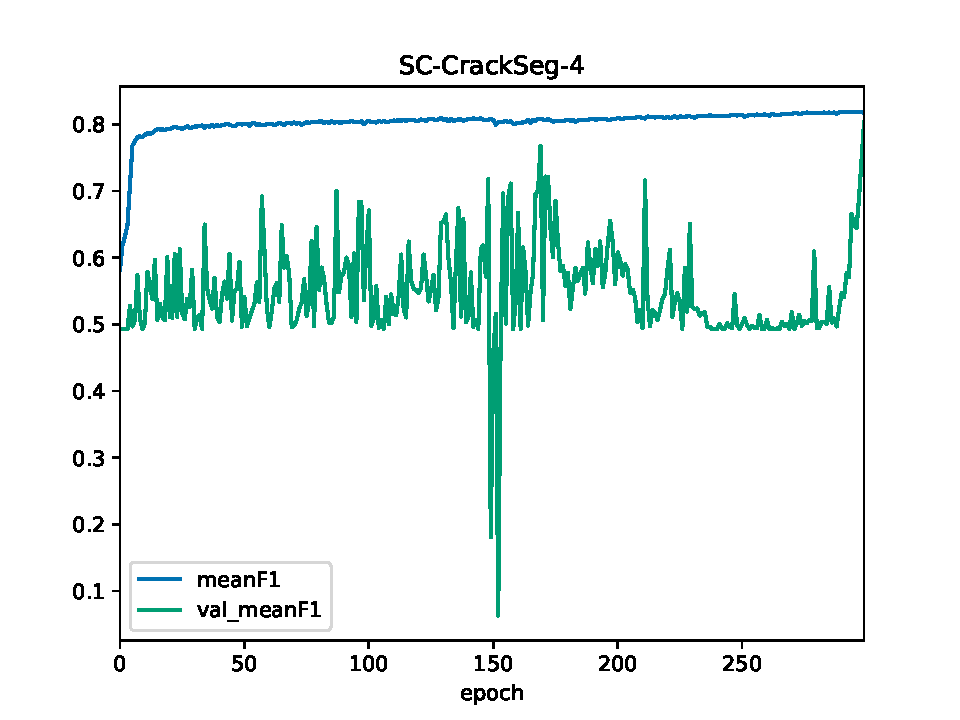
\includegraphics[width=0.3\textwidth]{res/crack-experiments-training-curves/sc-crackseg-4.pdf} \\
    \end{tabular}
    \caption{Train and test curves for SC-CrackSeg variations. Note the increased stability in models with DenSep modules (SDDNet, SC-CrackSeg-3, SC-CrackSeg-4).}
\end{figure}

Model stability also varied, with many models, especially SC-CrackSeg-2, often dropping in quality erratically. The introduction of the DenSep module appaeared to make models generally more stable. The larger models were, as expected, also more prone to overfitting.

Qualitative analysis revealed something interesting - only SDDNet and SC-CrackSeg-3 are capable of accurately segmenting specific crack boundaries. This performance does not appear to lead to major quantitative gains, but the distinction between "one crack" and "two cracks" could be significant in application context. SC-CrackSeg-3 may have this capability due to the enhanced global perspective provided by the deep branch and skip connections compared to SDDNet combined with the high-resolution detail provided by the skip connection, similarly to SDDNet.


\begin{figure}[htbp]
    \begin{tabular}{cccc}
        \begin{subfigure}[b]{0.23\textwidth}
            \centering
            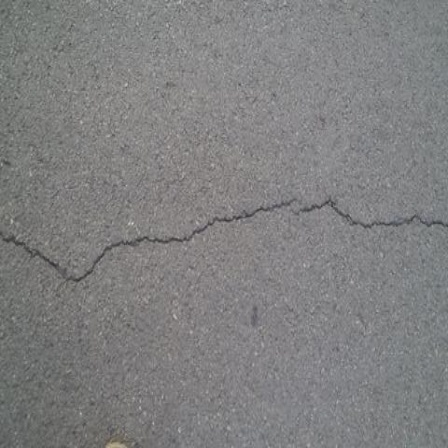
\includegraphics[width=\textwidth]{res/crackseg-experiment-qualitative/source.jpg}
            \caption{Source}
            \label{fig:crackseg-experiment-qualitative-source}
        \end{subfigure}
        \begin{subfigure}[b]{0.23\textwidth}
            \centering
            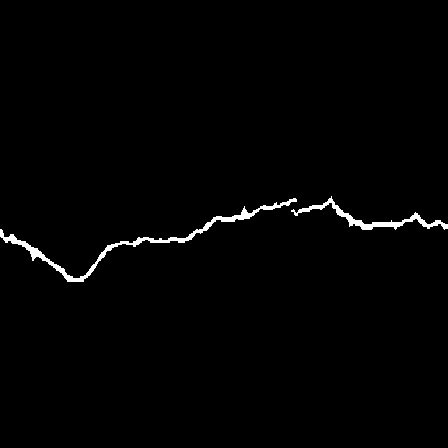
\includegraphics[width=\textwidth]{res/crackseg-experiment-qualitative/ground-truth.png}
            \caption{Ground Truth}
            \label{fig:crackseg-experiment-qualitative-ground-truth}
        \end{subfigure}
        \begin{subfigure}[b]{0.23\textwidth}
            \centering
            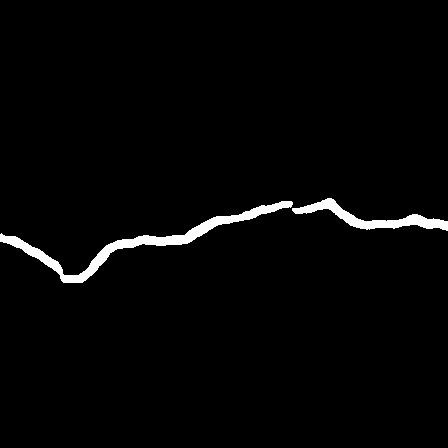
\includegraphics[width=\textwidth]{res/crackseg-experiment-qualitative/sddnet.png}
            \caption{SDDNet}
            \label{fig:crackseg-experiment-qualitative-sddnet}
        \end{subfigure}
        \begin{subfigure}[b]{0.23\textwidth}
            \centering
            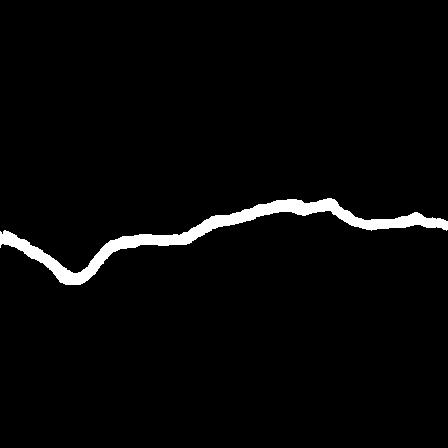
\includegraphics[width=\textwidth]{res/crackseg-experiment-qualitative/unet.png}
            \caption{U-Net}
            \label{fig:crackseg-experiment-qualitative-unet}
        \end{subfigure}
        \\
        \begin{subfigure}[b]{0.23\textwidth}
            \centering
            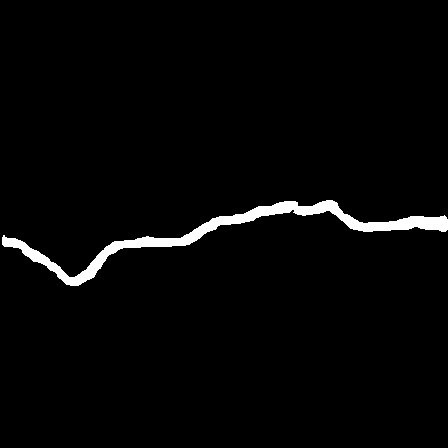
\includegraphics[width=\textwidth]{res/crackseg-experiment-qualitative/sc-crackseg-1.png}
            \caption{SC-CrackSeg-1}
            \label{fig:crackseg-experiment-qualitative-sc-crackseg-1}
        \end{subfigure}
        \begin{subfigure}[b]{0.23\textwidth}
            \centering
            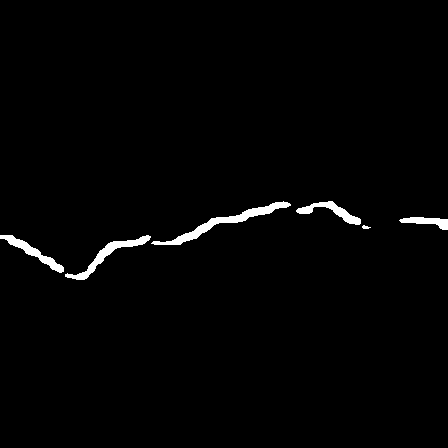
\includegraphics[width=\textwidth]{res/crackseg-experiment-qualitative/sc-crackseg-2.png}
            \caption{SC-CrackSeg-2}
            \label{fig:crackseg-experiment-qualitative-sc-crackseg-2}
        \end{subfigure}
        \begin{subfigure}[b]{0.23\textwidth}
            \centering
            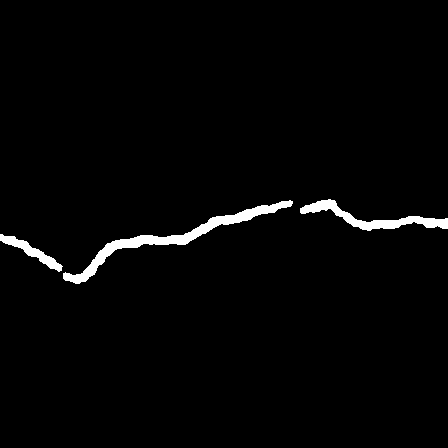
\includegraphics[width=\textwidth]{res/crackseg-experiment-qualitative/sc-crackseg-3.png}
            \caption{SC-CrackSeg-3}
            \label{fig:crackseg-experiment-qualitative-sc-crackseg-3}
        \end{subfigure}
        \begin{subfigure}[b]{0.23\textwidth}
            \centering
            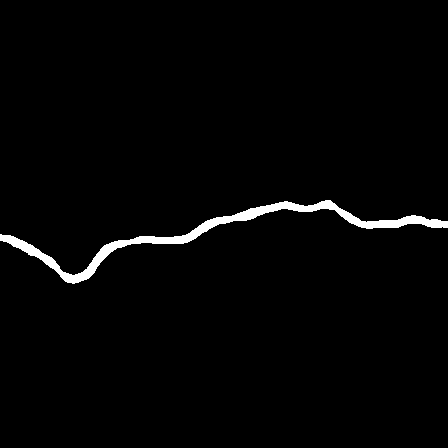
\includegraphics[width=\textwidth]{res/crackseg-experiment-qualitative/sc-crackseg-4.png}
            \caption{SC-CrackSeg-4}
            \label{fig:crackseg-experiment-qualitative-sc-crackseg-4}
        \end{subfigure}
    \end{tabular}
    \caption{Qualitative comparison of models on crack test set, displaying SC-CrackSeg-3 and SDDNet's ability to more finely segment crack components while maintaining quality.}
    \label{}
\end{figure}

Class balancing again achieved mixed success. While it initially appeared to have significant impact on performance, these were not consistent across experiments and random seeds. In fact, class imbalanced seemed to harm model performance in some areas, causing finely detailed crack segments to merged into a single large body [FIGURE]. High class imbalance specifically seemed to reduce model performance significantly.

\subsubsection*{Ablation Study}

Modifications in SC-CrackSeg-2 and SC-CrackSeg-3b were ablated. SC-CrackSeg-3b performed surprisingly strongly without the additional skip connection, though it still helps to improve performance and stabilise the model. SC-CrackSeg-2 originally contained more channels and additional layers in the shallow branch to increase processing of fine details, but ablation identified this increased complexity was unnecessary.

\begin{table}[]
    \begin{tabular}{|r|r|l|r|l|l|}
        \hline
        \multicolumn{1}{|l|}{\textbf{\begin{tabular}[c]{@{}l@{}}Deep \\ Conv \\ Layers/Set \\ Removed\end{tabular}}} & \multicolumn{1}{l|}{\textbf{\begin{tabular}[c]{@{}l@{}}Shallow \\ Conv \\ Layers/Set \\ Added\end{tabular}}} & \textbf{\begin{tabular}[c]{@{}l@{}}Reduced \\ Max\\ Channels\end{tabular}} & \multicolumn{1}{l|}{\textbf{Val mF1}} & \textbf{FLOPS} & \textbf{Parameters} \\ \hline
        0                                                                                                            & 0                                                                                                            &                                                                            & 0.807                                 & 1.4M           & 1.27M               \\ \hline
        1                                                                                                            & 0                                                                                                            &                                                                            & \textbf{0.808}                        & 1.22M          & 0.97M               \\ \hline
        0                                                                                                            & 1                                                                                                            &                                                                            & 0.798                                 & 1.42M          & 1.31M               \\ \hline
        1                                                                                                            & 1                                                                                                            &                                                                            & \textbf{0.808}                        & 1.24M          & 1.01M               \\ \hline
        2                                                                                                            & 0                                                                                                            &                                                                            & 0.799                                 & \textbf{1.14M} & \textbf{0.7M}       \\ \hline
        1                                                                                                            & 0                                                                                                            & Yes                                                                        & 0.807                                 & 1.19M          & 0.81M               \\ \hline
    \end{tabular}
\end{table}

\begin{table}[]
    \begin{tabular}{|l|l|r|l|l|}
        \hline
        \textbf{Skip Connection} & \textbf{DenSep Module} & \multicolumn{1}{l|}{\textbf{Val mF1}} & \textbf{FLOPS}        & \textbf{Parameters} \\ \hline
                                 &                        & 0.807                                 & \textbf{1.4M}         & \textbf{1.27M}      \\ \hline
        Yes                      &                        & 0.809                                 & 1.44M                 & 1.28M               \\ \hline
                                 & Yes                    & 0.811                                 & 2.12M                 & 1.5M                \\ \hline
        Yes                      & Yes                    & \textbf{0.812}                        & 2.16M                 & 1.51M               \\ \hline
    \end{tabular}
\end{table}

\subsection*{Conclusions}



While convential wisdom often states the strongest machine learning architectures are general, crack segmentation is an interesting example of a scenario where specifically tuned architectures can be significant. SC-CrackSeg and it's subsequent versions produced make select sacrifices in areas minimally impactful towards performance and applies specific optimisations for the crack segmentation task.

The lack of an effect provided by class balancing is surprising, particularly due to effectiveness observed in other papers \cite{liu_deepcrack_2019}. It appears the effect of class imbalance is model and scenario-dependent in crack segmentation. Perhaps more of an effect would have been observed in a more complex task than crack segmentation where a larger number of classes must be balanced. In crack segmentation, preducting further crack pixels is often the only way to further reduce loss, since there are only two classes.

We further discover the extreme effectiveness of SDDNet. DenSep blocks are simple, possess few parameters, and yet achieve extremely strong performance. Introduction of these blocks increases model stability and, when applied properly, the performance of SC-CrackSeg. In general, our experiments drive home that increased complexity is not necessary for the crack segmentation task, and may even be a hindrance, producing instability and overfitting. Though SDDNet is effective, our own SC-CrackSeg models may prove more effective in scenarios where computation count and model size.

In general, the lack of difference between widely varying architectures was surprising - many model's top F1 scores were within 0.01 of each other, despite varying qualitative results. This may be indiciation that there are further metrics in the crack segmentation task (such as number of cracks detected) not covered by traditional qualitative metrics, and that performance in terms of qualitative metrics has been largely saturated using the chosen architectures. Skip connections were found to have positive impact due to their ability to transfer feature resolution, while upsampling was found to be surprisingly ineffective, perhaps due to its tendency to increase model size and produce overfitting.

Ultimately, we introduce a number of competitive crack segmentation architectures in SC-CrackSeg and it's variations. We explore the effects of different architectural and external choices on performance in the context of crack segmentation.

% ------------------------------------------------------------------------------
% Unsupervised Domain Adaptation for Segmentation
% ------------------------------------------------------------------------------
\chapter{Adversarial Domain Adaptation for Transformer Segmentation}

\section{Background}

% TODO consider moving this section here from the very beginning (THEN ALSO CONSIDER MOVING FAST SEMANTIC SEGMETNATION TO THE FIRST CHAPTER AND FAST TRANSFORMER TO WHAT WILL PROBABLY BE THE LAST). Maybe also add like a "see section X.X for context"
% \subsection*{Transformers for Semantic Segmentation}

\subsection{Unsupervised Domain Adaptation}
Unsupervised Domain Adaptation (UDA) fundamentally seeks to address the lack of large amounts of high-quality training data for machine learning tasks. A subset of transfer learning, domain adaptaion explores how to transfer knowledge learned on a labelled source domain to an unlabeled target domain, where the two domains possess the same label space but contain a domain shift. This shift may be small (e.g. one city to another) or large (synthetic to real data). Formally, consider a source dataset $D_S$ consisting of inputs $X_S$ and labels $Y_S$ as samples from an overall distribution $P_S$. Similarly, a target set $D_T$ consists of images $X_T$ from a distribution $P_T$. Critically, the labels, $Y_T$, are not available. Due to the domain shift between the datasets, we can intuit $P_T \neq P_S$, bu that  $P_S$ will be a strong starting point for learning $P_T$ due to the similarity of the domains. UDA, then, involves strategies for moving from $P_S$ to $P_T$ \cite{wilson_survey_2020}, unsupervised labels for our true desired target $P_T$ are not available.

Many fundamentally different approaches to domain adaptation exist. Two in particular have become relevant to semantic segmentation: domain-adversarial learning and self-training. Domain adversarial learning is a subset of domain invariant feature learning \cite{wilson_survey_2020}, a UDA approach based on the intuition that a model will be most successful operating on features similar to those it was trained on. In other words, this UDA approach improves performance by encouraging the model to produce features from the target set similar to those in the source set. This is usually achieved by adding another parameter to the model loss, such as the statistical distance between the source and target model's feature distributions \cite{gretton_kernel_2006} \cite{sun_return_2015}. Recently, many publications instead implement an adversarial \cite{goodfellow_generative_2014} approach. One model is trained on the source/target dataset tasks, while another, the discriminator, takes features from the former as input and is trained to classify whether the features belong to the source or target dataset. The discriminator's loss is then negated and added to the original model's loss, training it to "trick" the discriminator. The intuition here is that producing source and target features that a neural network cannot distinguish is a more effective means of ensuring their similarity than traditional distances. This approach is known as domain adversarial learning \cite{ganin_domain-adversarial_2016}.

Self-training, or pseudo-labelling, is another common approach. It's intuition is that the highest quality, most "confident" predictions made by a source-trained model on target data will provide more valuable than non-valuable knowledge to the model \cite{wilson_survey_2020} \cite{kamnitsas_transductive_2021}. In essence, the source-trained model makes predictions on target samples, the most confident of these predictions - known as pseudo-labels - are added to the training set, and the cycle is repeated. How the confidence of a model is determined varies. Some studies use ensemble approaches, though many semantic segmentation techniques use the magnitude of a model's softmax output as a measure of confidence, where a greater softmax value is a more confident prediction \cite{zou_domain_2018}.

% TODO add example image explaining domain adversarial training 

\subsection*{UDA for Semantic Segmentation}

Both domain adversarail and self-training approaches have been applied to semantic segmentation, but must be adjusted due to the increased complexity of dense prediction. It is also critical to consider that semantic segmentation requires many predictions to be made per input, rather than a single one as in classification. \cite{hoffman_fcns_2016} was first in domain adversarial approaches, using FCN with a discriminator that took in feature space in "patches", where each patch represented the size of the model's receptive field. It was found passing all dense features to the discriminator simultaneously marginalised fine-grained detail in output predictions. This was addressed via a class distribution loss to encourage learning of rare classes. \cite{tsai_learning_2020} use an output-level discriminator combined with multiple feature-level discriminators, intuiting that the complex output space of segmentation should look similar between appraoches. \cite{wang_classes_2020} apply a fine-grained discriminator that produces class-wise logits to encourage the model to effectively transfer each class. \cite{michieli_adversarial_2020} combines a pixel-wise adversarial approach with self-training.

Self-training approaches have produced many state-of-the art results. Many contributions were made in \cite{zou_domain_2018}, who apply pseudo-labelling to segmentation by masking out (making the model ignore) all but the $r\%$ most confident correct pixel predictions in each image. Confidence is smeasured using softmax magnitude. A scheduling system is introduced to gradually increase $r$ as target predictions become more reliable. Class-balancing is also introduced to counteract the domination of easy-to-predict classes. ADVENT \cite{vu_advent_2019} found focusing training on low-confidence regions could boost performance, and \cite{li_bidirectional_2019} combines pseudolabelling with GAN image translation.
% TODO READ DACS FOR CHAPTER 3 AND WRITE ABOUT IT HERE

\subsection*{Vision Transformers in UDA}

Transformers are known to have extremely strong transfer learning capabilities \cite{radford_language_2019} \cite{wright_transformer_2020}. This extends to vision, where ViT \cite{dosovitskiy_image_2021} and SETR \cite{zheng_rethinking_2021} identified the effectiveness of pre-training on a large dataset like ImageNet before adapting to labelled segmentation data. Transferrable Vision Transformer (TVT) \cite{yang_tvt_2021} was the first to explore the domain adaptation abilities of vision transformers specifically, but did so in the classification space using ViT. It was found that ViT's zero-shot transferrability outperformed many state-of-the-art CNN-based techniques for domain adaptation. This was built on using an adversarial patch-wise discriminator that de-emphasises easy-to-disciminate patch weights, combined with a loss that maximises feature clustering \cite{chapelle_semi-supervised_2005}. Patch-wise feature alignment was also applied in \cite{wang_exploring_2021} for object detection.

\subsection*{DAFormer}

The domain transferability of general vision transformers and the state-of-the art performance of segmentation transformers like SegFormer had both been established by early 2022. However, there had been no exploration into combining these strengths.
The intuition here was that, just as vision transformers outperformed existing domain transfer approaches even with naive exmaples, there was a real possibility that a similar boost of performance could be achieved by segmentation transformers.

However, there are some differences between the application of domain adaptation in this context compared to in simpler computer vision approaches. For example, the fact that segmentation models output a number of predictions has required adaptations classificiation approaches where only one output is produced [CONSIDER EXPANDING ON THIS].

An intuitive approach to this problem would be to first apply a model like segformer to domain adaptation, first evaluating its performance in a naive setting (train on source, evaluate on target) and then using an approach tailored to domain adaptation. To avoid having to interact with many of the complexities brought on by moving from a convolutional to transformer architecture, a largely architecture-independent approach proven for segmentation, such as self-training [CITE] may be used. While this was the initial plan for this chapter of the thesis, it was also unfortunately the precise subject of the [MONTH] 2022 paper DAFormer by [AUTHOR] [CITE]. [SPECIFIC DESCRIPTION OF WHAT THEY DID AND HOW THEY DID IT, PLUS THE BONUS STUFF THEY DID LIKE IMAGENET FEATURE DISTANCE]. As I sought to explore novel concepts and approaches, I instead shifted focus onto the other popular means of performing domain adaptation - domain-adversarial training. Domain adversarial approaches were not explored in DAFormer due to the recent success of self-training in other research and the difficulty of implementing domain adversarial methods in segmentation transformers. The challenge comes primarily from the large changes that must be made to the training pipeline (adding a peripheral network with a separate training goal).

My final training pipeline was built on top of the DAFormer repository (itself built on the MMSegmentation framework). This allowed us to take advantage of the general framework changes necessary for domain adaptation, namely allowing for the input and preprocessing of multiple datasets.

% TODO some of this should go into methods, the rest should stay here as a more thorough explanation of DAFormer

\section{Methods}

\section{Experimental Results}

\section{Future Work}
A potentially promising approach would be to combine the class-level predictions of FADA \cite{wang_classes_2020} with the patch-wise discrimination approach of TVT \cite{yang_tvt_2021}. As the latter discusses, patches often represent class-level or global feature-level information. Therefore, enocuraging patches to learn domain-indiscriminate encodings while maintaining classes may allow adversarial approaches to overcome class marginalisation. However, this approach would require a means of labelling source and target patches with class information.

% ------------------------------------------------------------------------------
% Cross-Attention in Segmentation
% ------------------------------------------------------------------------------
\chapter{Efficient domain adaptation with lightweight transformers}

\section{Related Work}

\subsection{Efficient Transformers for Semantic Segmentation}

While the power of large vision transformers such as ViT and SegFormer trained on larger datasets is established, these properties do not properly present themselves in highly resource-constrained contexts, where the direct inductive biases of CNNs appear to win out. For instance, \cite{mehta_mobilevit_2022} identified a version of DEiT \cite{touvron_training_2021} with only around 6 million parameters, is outperformed by the traditional CNN-based MobileNetV3 \cite{howard_searching_2019}. Therefore, recent attempts have been made to produce lightweight transformer-based computer vision models, typically by combining the efficiency and inductive biases of CNNs with the strong global learning capability of transformers.

MobileViT \cite{mehta_mobilevit_2022} is an early popular appraoch. While existing approaches had explored introducing CNN-like inductive biases into transformer vision models [TODO CITE], MobileViT \cite{mehta_mobilevit_2022} used this concept to achieve lightweight inference. MobileViT, similar to SegFormer \cite{xie_segformer_2021}, has each block's input and output be in the form of a $\mathbb{R}^{H \times W \times C}$ tensor (where $H$ is height, $W$ is width, and $C$ is channels). However, instead of performing patch embedding, MobileViT blocks first use pointwise convolutions to transform input into a high-dimensional space $\mathbb{R}^{H \times W \times d}, d > C$, then unfold it into a $\mathbb{R}^{P \times N \times d}$ tensor, (where $P$ is product of patch dimensions $h \times w$ and $N$ is the patch number). Attention is then applied along individual pixels of each patch block [TODO FIGURE] before refolding to $\mathbb{R}^{H \times W \times D}$. This process of unfolding, folding, and processing, mirrors the same process that occurs during standard convolutions [CITE PYTORCH https://pytorch.org/docs/stable/generated/torch.nn.Unfold.html], transferring over the inductive biases of the operation while applying global receptive field. MobileViT outperforms CNNs and transformer networks while possessing significantly fewer parameters, using DeeplabV3's ASPP head \cite{chen_rethinking_2017} for segmentation output. Performance was also found to improve generalisability, the ability to perform on unseen datasets, compared to similarly-scaled transformer models.

\begin{figure}[ht!]
    \centering
    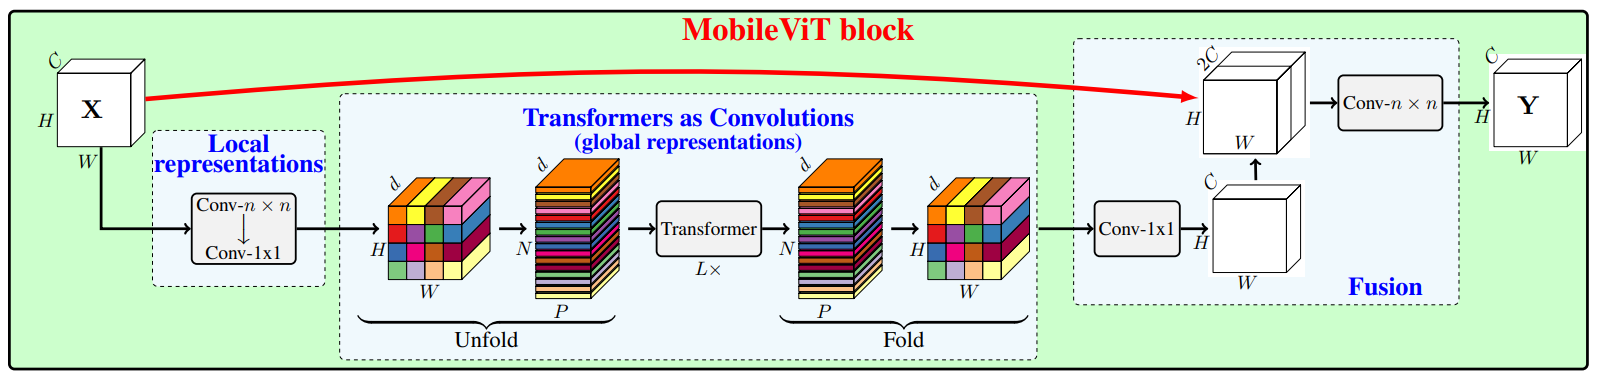
\includegraphics[width=\textwidth]{res/mobilevit-block.png}
    \caption{Architecture of a MobileViT block \cite{mehta_mobilevit_2022}. Features are input in CNN-like $H \times W \times C$ format, unfolded into a transformer input sequence, then re-folded into before being output.}
    \label{fig:mobilevit_block}
\end{figure}

Other approaches seeking efficiency combine CNNs and transformers more directly. Mobile-Former [TODO CITE] runs mobilenet and transformer blocks in parallel to achieve performance and efficiency gains over MobileNetV3, though at a still high number of FLOPs and parameters. More recently, TopFormer \cite{zhang_topformer_2022} focuses specifically on fast transformer-based segmentation by using a feature pyramid-like design. First, MobileNet blocks are used to build a multiscale feature pyramid to reduce input dimension (down to $\frac{1}{64}$ of target size). All block output tokens are then average pooled to the size of the smallest and concatenated. After patch embedding, these tokens are passed through a standard vision transformer. The tokens are then reshaped, de-concatenated, and upsampled before being combined with their original counterparts. The final tokens are then combined in a convolution-based gradual upsampling process, similar to U-Net \cite{ronneberger_u-net_2015} and approaches discussed in chapter 2. The benefit of this approach is tow-fold: CNN inductive biases are applied during downsampling and upsampling and the global receptive field of transformers is applied at low convolutional cost due to the small input size. The transformer's attention also enables the sharing of features across resolutions. TopFormer achieves particularly strong results on the challenging ADE20K dataset, known for its complex scenery.

% "MobileNet convolutional" CHECK IF IT SHOULD BE BOTTLENECK?


\FloatBarrier

% \begin{figure}
%     \centering
%     \includegraphics[width=\textwidth]{}
%     \caption{example figure}
%     \label{fig:example-fig}
% \end{figure}

\chapter{Conclusion}
\section{Future Work}

% \section{acknowledgement}
% Supervisors - Aneesh & Sonny

% ******************
\bibliography{thesis}{}
\bibliographystyle{IEEEtran}

\end{document}